\documentclass{sig-alternate}
\usepackage{url}
\usepackage{graphicx}
\usepackage{subfigure}
\usepackage{hyperref}
\usepackage{url}
\usepackage{times}
\usepackage{balance}
\usepackage{xspace}
\usepackage{xfrac}

\begin{document}

\newcommand{\todo}[1]{\textbf{TODO}\footnote{\textbf{TODO:} #1}}

\newcommand{\ghtorrent}{ \textsc{ght}orrent\xspace}
\newcommand{\api}{\textsc{api}\xspace}

\title{An Exploratory Study of the Pull-based Software Development Model}
\numberofauthors{3}

\author{
\alignauthor
Georgios Gousios\\
       \affaddr{Delft University of Technology}\\
       \affaddr{Delft, The Netherlands}\\
       \email{G.Gousios@tudelft.nl}
\alignauthor
Martin Pinzger\\
       \affaddr{University of Klagenfurt}\\
       \affaddr{Klagenfurt, Austria}\\
       \email{martin.pinzger@aau.at}
\alignauthor
Arie van Deursen\\
       \affaddr{Delft University of Technology}\\
       \affaddr{Delft, The Netherlands}\\       
       \email{Arie.vandeursen@tudelft.nl}
}

\maketitle

\begin{abstract}

  The advent of distributed version control systems has led to the development
  of a new paradigm for distributed software development; instead of pushing
  changes to a central repository, developers pull them from other repositories
  and merge them locally. Various code hosting sites, notably Github, have
  tapped on the opportunity to facilitate pull-based development by offering
  workflow support tools, such as code reviewing systems and integrated issue
  trackers. In this work, we explore how pull-based software development works,
  first on the {\sc ght}orrent corpus and then on a carefully selected sample of 291
  projects. We find that the pull request model offers fast turnaround,
  increased opportunities for community engagement and decreased
  time to incorporate contributions. We show that a relatively
  small number of factors affect both the decision to merge a pull request and
  the time to process it. We also examine the reasons for pull request
  rejection and find that technical ones are only a small minority.

\end{abstract}

\category{D.2.7}{Software Engineering}{Distribution, Maintenance, and Enhancement}[Version control]
\category{D.2.9}{Software Engineering}{Management}[Programming teams]

\terms{Management}

\keywords{pull-based development, pull request, distributed software development,
empirical software engineering}

\section{Introduction}

%Several code hosting sites, including Github and BitBucket, tapped on the
%opportunity to make the pull-based development model more accessible to
%programmers. A unique characteristic of such sites is that they allow any user
%to fork any public repository. The clone creates a public project that belongs
%to user that cloned it, so the user can modify the repository without being part
%of the development team. What is more important is they automate the selective
%contribution of commits from the clone to the source, through pull requests. As
%mentioned earlier, pull requests are not unique to code hosting sites; in fact,
%the Git software distribution includes the \textsf{git-request-pull} utility
%which provides the same functionality at the command line. Github
%improved\footnote{Not everyone agrees:
%\url{https://github.com/torvalds/linux/pull/17}} this process significantly by
%integrating code reviews, discussions and issues, thus effectively lowering the
%entry barrier for casual contributions. Combined, cloning and pull requests
%create a new development model, where changes are pushed to the project
%maintainers and go through code review by the community before being integrated. 
%

Pull-based development is an emerging paradigm for distributed software
development. As more developers appreciate isolated
development and branching~\cite{Bird12}, more projects, both closed source and,
especially, open source, are being migrated to code hosting sites such as Github
and Bitbucket with support for pull-based development~\cite{Barr12}. A unique
characteristic of such sites is that they allow any user to clone any public
repository. The clone creates a public project that belongs to the user that
cloned it, so the user can modify the repository without being part of the
development team. Furthermore, such sites automate the selective
contribution of commits from the clone to the source through pull requests. 

Pull requests as a distributed development model in general, and as implemented
by Github in particular, form a new method for collaborating on distributed
software development. The novelty lays in the decoupling of the development
effort from the decision to incorporate the results of the development in the
code base. By separating the concerns of building artifacts and integrating
changes, work is cleanly distributed between a contributor team that submits, often
occasional, changes to be considered for merging and a core team that oversees
the merge process, providing feedback, conducting tests, requesting changes, and
finally accepting the contributions.

Previous work has identified the processes of collaboration in distributed
development through patch submission and acceptance \cite{MOCKU02, Bird07,
Weiss08}. There are many similarities to the way pull requests work; for
example, similar work team structures emerge, since typically pull requests go
through an assessment process. What pull requests offer in addition is
process automation and centralization of information. With pull requests, the
code does not have to leave the revision control system, and therefore it can be
versioned across repositories, while authorship information is effortlessly
maintained. Communication about the change is context-specific, being rooted on
a single pull request. Moreover, the review mechanism that Github incorporates
has the additional effect of improving awareness~\cite{Dabbi12}; core developers
can access in an efficient way all information that relates to a pull request
and solicit opinions of the community (``crowd-source'') about the merging
decision.

A distributed development workflow is effective if pull requests are eventually
accepted, and it is efficient if the time this takes is as short as possible.
Advancing our insight in the effectiveness and efficiency of pull request
handling is of direct interest to contributors and developers alike. The goal of
this work is to obtain a deep understanding of pull request usage and to analyze
the factors that affect the efficiency of the pull-based software development
model. Specifically, the questions we are trying to answer are: 

\begin{description}
  
  \item[RQ1] How popular is the pull based development model?

  \item[RQ2] What are the lifecycle characteristics of pull requests?
    
  \item[RQ3] What factors affect the decision and the time required to merge a pull request?

  \item[RQ4] Why are some pull requests not merged?

\end{description}

Our study is based on data from the Github collaborative development forge, as
made available through our {\sc ght}orrent project~\cite{G13}. Using it, we
first explore the use of almost 2 million pull requests across all projects in
Github. We then examine 291 carefully selected Ruby, Python, Java and Scala
projects (in total, 166,884 pull requests), and identify, using  qualitative and
quantitative analysis, the factors that affect pull request lifetime, merging
and rejection. 

%The results show that
%pull request acceptance is very high (> 80\%), while the majority of
%pull requests are merged within a day.
%On the other hand, pull request \emph{merge time} can be predicted with
%reasonable accuracy (> 70\%), while it is mostly dependent on the ensuing
%discussion, the size of the project and its test coverage. Both results can be
%utilized by developers to submit better pull requests and project managers to
%prioritize pull requests, while it opens new opportunities for research, such as
%building automated tools for pull request triaging.

\section{Background} \label{sec:bg}

Since their appearance in 2001, distributed version control systems ({\sc
dvcs}), notably Git~\cite{Chaco09}, have revolutionized the way distributed
software development is carried out. Driven by pragmatic needs, most {\sc dvcs}s
were designed from scratch to work as advanced patch management systems, rather
than versioned file systems, the then dominant version control paradigm. In most
{\sc dvcs}s, a file is an ordered set of changes, the serial application of
which leads to the current state. Changes are stamped by globally unique
identifiers, which can be used to track the commit's content across
repositories. When integrating changes, the change sets can originate from a
local filesystem or a remote host; tools facilitate the acquisition and
application of change sets on a local mirror. The distributed nature of {\sc
dvcs}s enables a pull-based development model, where changes are offered to a
project repository through a network of project forks; it is up to the
repository owner to accept or reject the incoming pull requests.

The purpose of distributed development is to enable a potential
\emph{contributor} to submit a set of changes to a software project managed by a
\emph{core team}. The development models afforded by {\sc dvcs}s are a superset
of those in centralized version control environments~\cite{Shiha12,Bird09}.
With respect to receiving and processing external contributions, the following
strategies can be employed with {\sc dvc}s:

\textbf{Shared repository.}
    The core team shares the project's repository, with read and write
    permissions, with the contributors. To work, contributors clone it locally,
    modify its contents, potentially introducing new branches, and push their
    changes back to the central one. To cope with multiple versions and multiple
    developers, larger projects usually adopt a {\em branching model}, i.e., an
    organized way to inspect and test contributions before those are merged to
    the main development branch~\cite{Bird12}. 
    
    %While the exact details depend on the
    %project requirements, usually branching models include feature branches,
    %where developers implement new features and fix bugs, and release branches,
    %which store the state of each project release. After the work has finished
    %on a feature branch its contents are merged appropriately to release
    %branches and to the project master branch.

\textbf{Pull requests.}
    The project's main repository is not shared among potential contributors;
    instead, contributors \emph{fork} (clone) the repository and make their
    changes independent of each other. When a set of changes is ready to be
    submitted to the main repository, they create a \emph{pull request}, which
    specifies a local branch to be merged with a branch in the main
    repository. A member of the project's core team is then responsible to
    inspect the changes and pull them to the project's master branch. If changes
    are considered unsatisfactory, more changes may be requested; in that case,
    contributors need to update their local branches with new commits.
    Furthermore, as pull requests only specify branches from which certain
    commits can be pulled, there is nothing that forbids their use in the shared
    repository approach (\emph{cross-branch pull requests}). An overview of the
    pull request process can be seen in Figure~\ref{fig:pullreq-process}.

    \begin{figure}[t]
      \begin{center}
        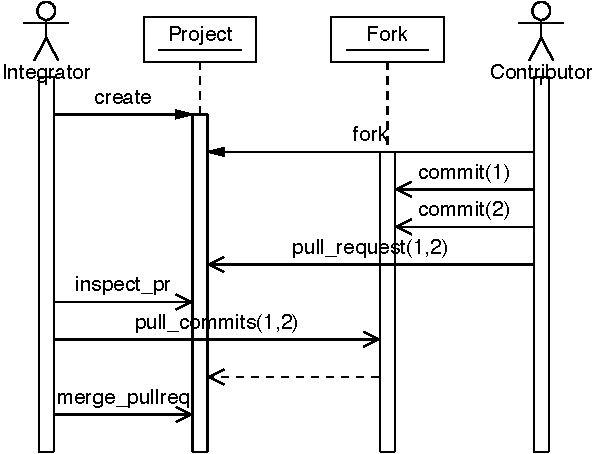
\includegraphics[scale=0.5]{pullreq}
      \end{center}
      \caption{The pull request process.}
      \label{fig:pullreq-process}
    \end{figure}

\subsection{Pull requests in Github}

Github supports all types of distributed development outlined above; however,
pull requests receive special treatment. The site is tuned to allow easy forking
of projects by contributors, while facilitating the generation of pull requests
through automatic comparison of project branches.
Github's pull request model follows the generic pattern presented above; in
addition it provides tools for contextual discussions and in-line code reviews.
An example pull request on Github can be seen in Figure~\ref{fig:pullreq-scr}.

\begin{figure}[t]
  \centering
   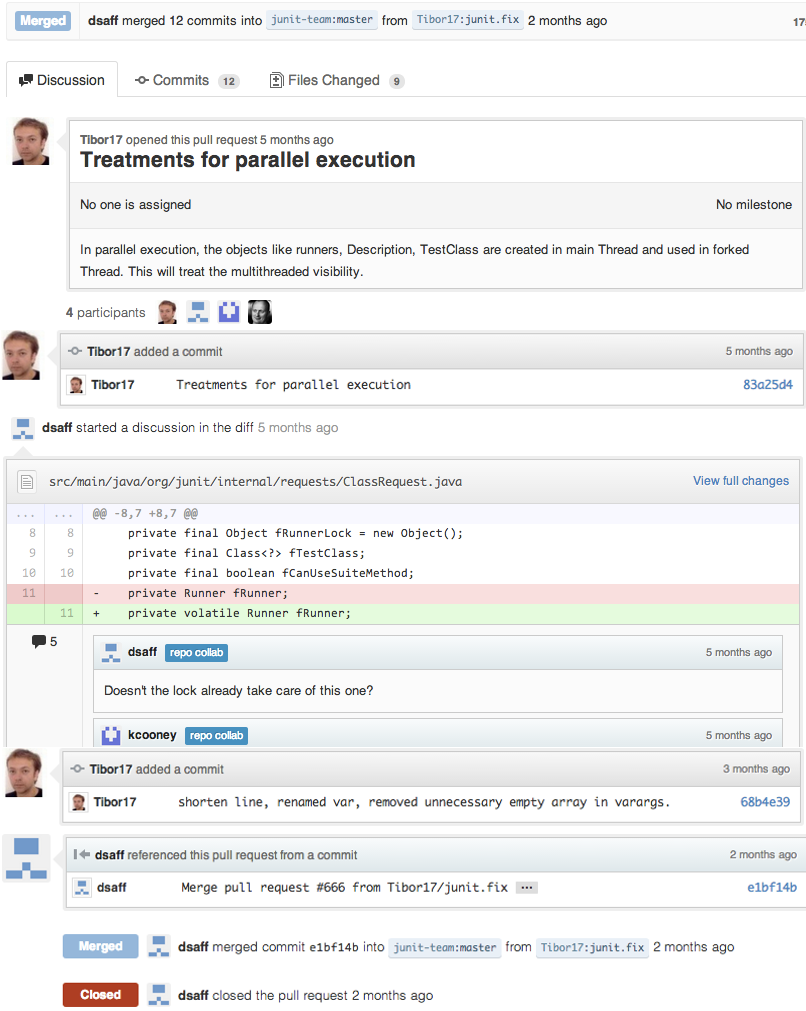
\includegraphics[scale=0.29]{pullreq-scr.png}
   \caption{An example Github pull request (667 from junit-team/junit --- edited for space). The
   participants first interact in a code review, the result of which is
   a new commit. The second reviewer then merges the pull request}
   \label{fig:pullreq-scr}
\end{figure}

A Github pull request contains a branch (local or in another repository) from
which a core team member should pull commits from. Github automatically
discovers the commits to be merged and presents them in the pull request. By
default, pull requests are submitted to the base (``upstream'' in Git parlance)
repository for inspection. The
inspection is either a code review of the commits submitted with the pull
request or a discussion about the features introduced by the pull request. Any
Github user can participate to both types of inspection. As a result of the
inspection, pull requests can be updated with new commits or be closed as
redundant, uninteresting or duplicate. In case of an update, the contributor
creates new commits in the forked repository, while Github automatically
updates the displayed commits. The code inspection can then be repeated on the
refreshed commits.

When the inspection process finishes and the pull requests are deemed
satisfactory, the pull request can be merged. A pull request can only be merged
by core team members. The versatility of Git enables pull requests to be
merged in three ways, presented below sorted by the amount of preservation of
the original source code properties:

\textbf{1. Through Github facilities.}
    Github can automatically verify whether a
    pull request can be merged without conflicts to the base repository. When a
    merge is requested, Github will automatically apply the commits in the pull
    request and record the merge event. All authorship and history information
    is maintained in the merged commits.

\textbf{2. Using Git merge.} When a pull request cannot be applied cleanly or
    when project-related policies do not permit automatic merging, a pull
    request can be merged using plain Git utilities, using the following
    techniques: 

    \begin{itemize}

      \item \emph{Branch merging:} The branch in the forked repository
        containing the pull request commits is merged into a branch in the base
        repository. Both history and authorship information are maintained, but
        Github cannot detect the merge in order to record a merge
        event~\cite[Chapter 3.2]{Chaco09}. 

      \item \emph{Cherry-picking:} Instead of merging all commits, the merger
        picks specific commits from the remote branch, which then applies to the
        upstream branch. The unique commit identifier changes, so exact history
        cannot be maintained, but authorship is 
        preserved~\cite[Chapter 5.3]{Chaco09}.
    
    \end{itemize}

    A technique that complements both of the above is \emph{commit
    squa\-shing}: if the full history is not of interest to the project,
    several consecutive commits are combined into a single one on the pull request
    branch, which can then be merged or cherry-picked to the upstream branch. In
    this case, the author of the commit is different from the person that
    applied the commit~\cite[Chapter 6.4]{Chaco09}. Both cherry-picking and
    commit squashing are by-products of Git's support for re-ordering commits
    (\emph{rebase})~\cite[Chapter 3.6]{Chaco09}.

\textbf{3. Committing the patch.} 
  The merger creates a textual difference between the upstream and the pull
  request branch, which she then applies to the upstream branch. Both history and
  authorship information are lost.

As the project branches are updated in a distributed manner, the changes in a
pull request may interfere with new changes in the project's main branch.
Merging such a pull request will result in \emph{conflicts}. Github
automatically detects conflicting pull requests and marks them as such.
Conflicts can be resolved by either the contributor or a core team member;
however, pull request etiquette dictates that the contributor takes care of
bringing the pull request back into a state where there are no conflicts. The
conflict resolution process involves pulling new commits from the project's main
repository, making changes to eliminate the conflicts and
extending the pull request with the resulting conflict eliminating commits.

Issues and pull requests are dual on Github; for each pull request, an issue is
opened automatically. Commits can also be attached to issues to convert them to
pull requests (albeit with external tools). This duality enables the core team
to treat pull requests as work items, which can be managed using the same
facilities used for issues. Moreover, issue discussions can include links to
pull requests and vice versa, while specific commit message formats can be used 
to automatically close issues or pull requests when commits are
merged to the project's main branch.

The open nature of Github's pull requests lends itself to a variety of usage
patterns. Except from basic patch submission, pull requests can be used as a
requirements and design discussion tool\footnote{Github uses this internally:
\url{https://github.com/blog/1124-how-we-use-pull-requests-to-build-github}} or
as a progress tracking tool towards the fulfillment of a project
release.\footnote{\url{https://github.com/blog/831-issues-2-0-the-next-generation}} In
the first case, a pull request serves as a discussion board for soliciting the
opinions of other developers while a new feature is being implemented. In the
second case, pull requests are associated with milestones in Github's issue
tracker.

\section{Research Design}
\label{sec:resdesign}

The main focus of this study is to understand and explain how pull requests are
used by projects to enable collaboration. To answer our research questions, we
use a sequential mixed-methods approach, a procedure for
collecting, analyzing, and integrating both quantitative and qualitative data at
some stage of the research process within a single study for the purpose of
gaining a better understanding of the problem~\cite{Ivank06}. For specific 
research questions, we first explore the domain quantitatively,
and then highlight interesting cases by exploring cases qualitatively.
Below, we present how we approached each research question.

{\bfseries RQ1} To assess the popularity of the pull-based development model, we
provide and analyze descriptive statistics on the use of pull requests in Github.
In particular, we investigate such questions as how many projects actually make
use of pull requests, how many of the projects are original repositories
(versus, e.g., forks), and how pull requests relate to Github's issue tracking
facilities. The outcomes are presented in Section~\ref{sec:github}.

{\bfseries RQ2 and RQ3}
Identifying the lifecycle characteristics of pull requests and determining the
factors that affect them calls for a dedicated dataset of projects that have a
sufficiently long history of using pull requests. This dataset is described in
Section~\ref{sec:expdata}.

Given this dataset, we answer {\sc rq2} and {\sc rq3} by determining a set of
suitable candidate features through consultation of related work in the fields
of patch submission, bug triaging, code reviewing and distributed collaboration.
Then, we clean it up through cross-correlation analysis to obtain a set of
features with maximum predictive power. Using the data from the extracted
features, we perform a detailed statistical analysis of pull request
characteristics to answer {\sc rq2} (Section~\ref{sec:pullreqchar}).

Next, we use machine learning to retrieve the dominant
features. Prior to running the classification algorithms, we automatically labeled
each pull request with an outcome factor; in the case of the \textsf{merge
decision} classification task, the label signifies whether the pull request has
been merged. For the \textsf{merge time} task, we first filter out pull requests
that have not been merged and then split the remaining data points into three
classes (\textsf{hour}, \textsf{day}, \textsf{more than a day}) according to the time
required to merge the pull request. The split points were chosen to reflect the
results of {\sc rq2}, and split the available data points into roughly equally
sized bins.

At a high level, the process to retrieve the dominant features for both
classification tasks consists of two steps.  First, we run each dataset through
6 classification algorithms, namely Random Forests (\texttt{randomforest}),
variants of Logistic Regression (\texttt{logregr}) (binary for the \textsf{merge
decision} task, multinomial for the \textsf{merge time} task) and Na\"ive Bayes
(\texttt{naivebayes}), Support Vector Machines (\texttt{svm}), decision trees
(\texttt{dtree}) and AdaBoost with decision trees (\texttt{adaboost}). We used
those algorithms as they are known to perform well in large
datasets~\cite{Lessm08} and have been used in previous work involving prediction
models~\cite{Giger12}. We do not perform any additional tuning to the
classification algorithms. We only report results on the first three, as those
performed best. Then, we select the best classifier and apply a
classifier-specific process to rank features according to their importance in
the classification process. 

To evaluate the classification performance, we use the Accuracy ({\sc acc}) and
Area Under the receiver operating characteristic Curve ({\sc auc}) metrics. To
select the appropriate classification algorithm, we run a 10-fold random
selection cross-validation and aggregate the mean values for each classification
metric. At each iteration, the algorithm randomly samples half of the
available data points, trains a classifier with 90\% percent of the input and
uses it to predict the remaining 10\%. The 10-fold run results also allowed us to
evaluate the metric stability across runs (Section~\ref{sec:accrej}).

{\bfseries RQ4} To examine why some pull requests are not merged, we
qualitatively analyze a set of randomly chosen non-merged pull requests in
depth. We use open coding (a grounded theory tool) to come up with an inclusive
set of reasons of why pull requests are not merged as follows: the first author
read the pull request discussion on Github for randomly selected pull requests
and summarized the reasons for closing them into one sentence per sample; during
a second pass, the descriptions were aggregated and codes were extracted. To
validate the identified codes, all three authors applied them on a different set
of pull requests, compared results, identified inconsistencies and retrofitted
the initial selection of codes. The final set of codes was then applied on a
third sample which we used to draw results from. The sampling process
is described in Section~\ref{sec:qualdata}.

\section{Data}

\subsection{Github data}
\label{sec:ghtorrent}

We used Github data as provided through our {\sc ght}orrent project \cite{G13},
an off-line mirror of the data
offered through the Github {\sc api}. The Github {\sc api} 
data come in two forms; a streaming
data flow lists events, such as forking or creating pull requests, happening on
repositories in real time, while a static view contains the current state of
entities. To obtain references to the roots of the static view entities, the
{\sc ght}orrent project follows the event stream. From there, it applies a
recursive dependency-based parsing approach to yield all data offered through
the {\sc api}. The data is stored in unprocessed format, in a Mongo{\sc db}
database, while metadata is extracted and stored in a My{\sc sql} relational
database. The {\sc ght}orrent dataset covers a broad range of development
activities on Github, including pull requests and issues. The project
has been collecting data since February 2012. Up to August 2013,
1.9 million pull requests from more than two hundred thousand projects
have been collected.

\subsection{Pull request project sample}
\label{sec:expdata} 

\textbf{Project selection.} To make the analysis practical, while avoiding to
examine toy projects, we use a dataset consisting of all projects for which
\ghtorrent recorded more than 200 pull requests in the period between February
2012 and August 2013. The initial selection resulted in 374 projects. The
following criteria were then applied to exclude projects from the initial
selection:

\begin{itemize}

  \item Projects should include tests. To measure the effect of testing on pull
    request acceptance, we could only use projects that include tests which we
    could measure reliably. For that, we exploited the convention-based project
    layout in the Ruby (Gem), Python, Java and Scala (both Maven) language
    ecosystems, so our project selection was limited to those languages. 

  \item Projects should have at least one commit coming from a pull request, to
    ensure that the project is open to external contributions and that pull
    requests are not just used by developers inside the project.

  \item Projects should be developing software frameworks or applications,
    rather than documentation or programming languages. We excluded
    documentation projects, because we are interested in distributed software
    development. We excluded programming language implementation projects
    because we wanted to avoid cases where the developed programming language's
    core library was overshadowing the metrics of the actual implementation.
    This is especially true for the 5 Ruby implementations hosted on Github.

\end{itemize}

After selection, the full history (including pull requests, issues and commits)
of the included projects was downloaded and features were extracted by querying
the {\sc ght}orrent databases and analyzing each project's Git repository. 
Furthermore, for these selected projects we collected all merges and the values for all factors that we use in our machine learning experiment, as described below.

\textbf{Merge detection.} To
identify merged pull requests that are merged outside Github, we resorted to the following heuristics, listed here in order of application:

\begin{enumerate}

  \item At least one of the commits associated with the pull request appears in
    the target project's master branch. 

  \item A commit closes the pull request (using the \texttt{fixes:} convention
    advocated by Github) and that commit appears in the project's master branch.
    This means that the pull request commits were squashed onto one commit and
    this commit was merged.

  \item One of the last 3 (in order of appearance) discussion comments contain a
    commit unique identifier, this commit appears in the project's master branch
    and the corresponding comment can be matched by the following regular
    expression:

    \begin{small}
    \texttt{(?:merg|appl|pull|push|integrat)(?:ing|i?ed)}
    \end{small}
  \item The latest comment prior to closing the pull request matches the 
    regular expression above.

\end{enumerate}

If none of the above heuristics identifies a merge, we mark the pull request
as unmerged. 

After creating the data files, we investigated projects where the pull request
merge ratio was significantly less than the one we calculated across Github
(73\%), and in any case less than 40\%, as this means that our heuristics are not
good enough for this project. This way, we filtered out 2 projects, which we did not
replace.

The final dataset consisted of 291 projects (99 Python, 91 Java, 87 Ruby, 14
Scala) and 166,884 pull requests (59,970; 55,468; 43,870 and 7,576 for Python,
Ruby, Java and Scala projects respectively). Both distributions are
representative of the contemporary popularity of each respective programming
language on both Github and other sites.

%Figure~\ref{fig:wordcloud} presents the project names in relative size to the
%pull requests included per project in the dataset. 
%
%\begin{figure}
%  \begin{center}
%    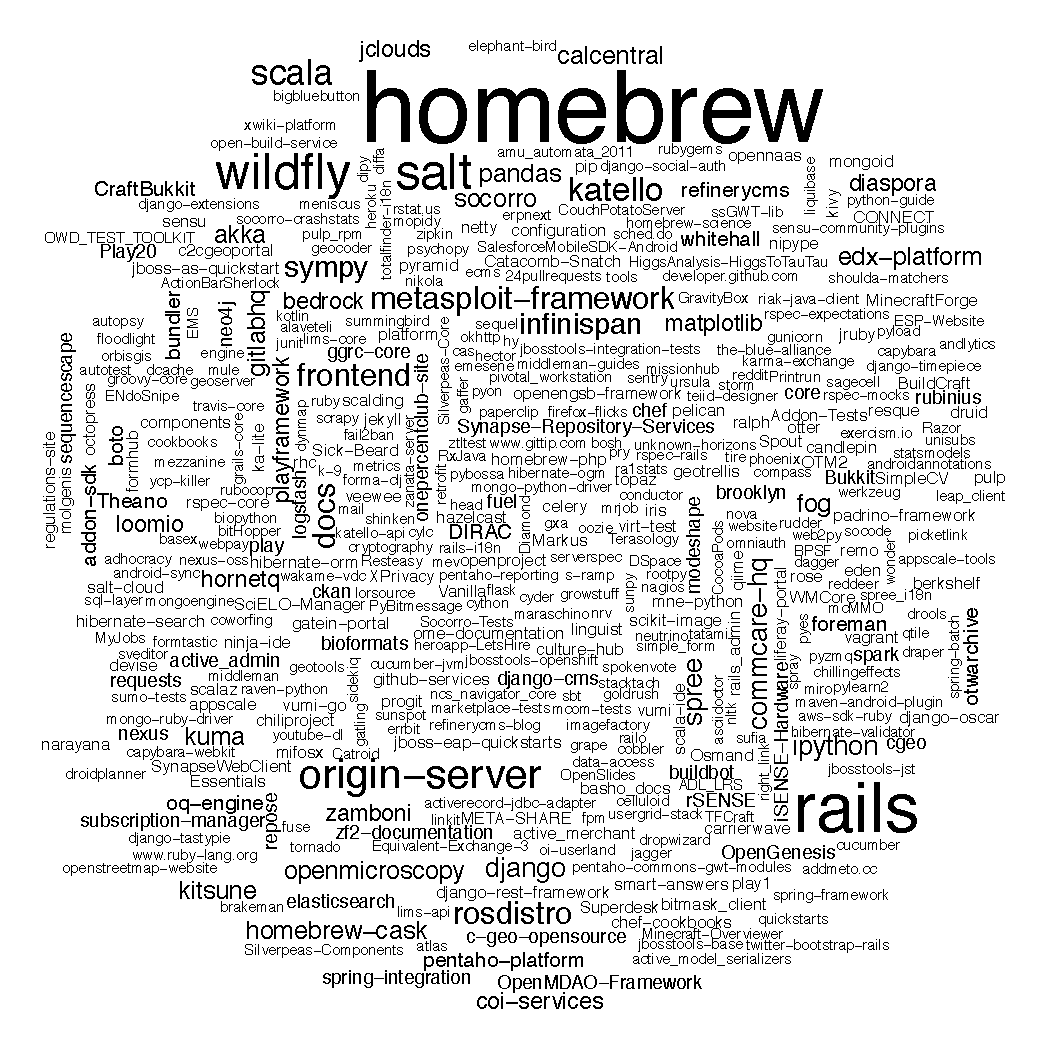
\includegraphics[scale=0.7]{wordcloud.pdf}
%  \end{center}
%  \caption{Projects in our dataset. Text size is relative to the number of
%  included pull requests.}
%  \label{fig:wordcloud}
%\end{figure}

\textbf{Feature Extraction.} The feature selection was based on prior work in the areas of patch submission and acceptance~\cite{Nagap05,Bird07a,Weiss08,Baysa12}, 
code reviewing~\cite{Rigby13}, bug
triaging~\cite{Anvik06, Giger10} and also on semi-structured interviews of
Github developers~\cite{Dabbi12, Pham13, McDon13}. The selected features are split
into three categories:

  \emph{Pull request characteristics.} These features attempt to quantify the
  impact of the pull request on the affected code base. When examining external
  code contributions, the size of the patch is affecting both acceptance and
  acceptance time~\cite{Weiss08}. There are various metrics to determine the
  size of a patch that have been used by researchers: code churn~\cite{Nagap05,
  Ratzi07}, changed files~\cite{Nagap05} and number of commits~\cite{Fluri07}.
  In the particular case of pull requests, developers reported that the presence
  of tests in a pull request increases their confidence to merge
  it~\cite{Pham13}. To investigate this, we split the churn feature into two
  features, namely \texttt{src\_churn} and \texttt{test\_churn}. The
  number of participants has been shown to influence the time to process of code
  reviewing~\cite{Rigby13}. Finally, through our own experience analyzing pull
  requests, we have found that in many cases conflicts are reported explicitly
  in pull request comments while in other cases pull requests include links to
  other related pull requests.

  \emph{Project characteristics.} These features quantify how receptive to pull
  requests the project is. If the project's process is open to external
  contributions, then we expect to see an increased ratio of external
  contributors over team members. The project's size may be a detrimental factor
  to the speed of processing a pull request, as its impact may be more difficult
  to assess. Also, incoming changes tend to cluster over time (the ``yesterday's
  weather'' change pattern~\cite{Girba04}), so it is natural to assume that pull
  requests affecting a part of the system that is under active development will
  be more likely to merge. Testing plays a role in speed of processing;
  according to~\cite{Pham13}, projects struggling with a constant flux of
  contributors use testing, manual or preferably automated, as a safety net to
  handle contributions from unknown developers.

  \emph{Developer.}  Developer-based features quantify the influence that the
  person who created the pull request has on the decision to merge it and the
  time to process it. In particular, the developer who created the patch has
  been shown to influence the patch acceptance decision~\cite{Jeong09}. To
  abstract the results across projects with different developers, we include
  features that quantify the developer's track record~\cite{Dabbi12}, namely the
  number of previous pull requests and their acceptance rate; the former has
  been identified as a strong indicator of pull request quality~\cite{Pham13}.
  Bird et al.~\cite{Bird07}, presented evidence that social reputation has an
  impact on whether a patch will be merged; in our dataset, the number of
  followers on Github can be seen as a proxy for reputation.

All features are calculated at the time a pull request has been closed or
merged, to evaluate the effect of intermediate updates to the pull request as a
result of the ensuing discussion. Features that contain a temporal dimension in
their calculation (e.g., \texttt{team\_size} or
\texttt{commits\_on\_files\_touched}) are calculated over the three-month time
period before the pull request was opened.

The initial selection contained 25 features. To check whe\-ther the selected
features are sufficiently independent, we
conducted a pair-wise correlation analysis using the Spearman rank correlation
($\rho$) metric across all features. We set a threshold of $\rho = 0.7$, above
which we eliminated features. Using this cutoff, we
removed 2 features, \texttt{asserts\_per\_kloc} and
\texttt{test\_cases\_per\_kloc} as they where very strongly correlated ($\rho >
0.92$) with the included \texttt{test\_lines\_per\_kloc} feature. We also
removed features that could not be calculated reliably at the time a pull
request was done (\texttt{followers} and \texttt{stars}).
%\footnote{The Github
%{\sc api} does not report a timestamp on when a user followed another user, or
%when a user stared a project, so it is impossible to know how many followers a
%user had or stars a project had at a specific time instance.} 
Finally, we
merged similar features (i.e. \texttt{doc\_files} and \texttt{src\_files} were merged to \texttt{files\_changed}). 

The post processing phase left us with 15 features, which can be seen in
Table~\ref{tab:features}. 
%The cross-correlation analysis result for the
%selected features can be seen in Figure~\ref{fig:crosscor}. 
In general, very few
features are correlated at a value $\rho > 0.2$, while only two,
\texttt{src\_churn} and \texttt{files\_chan\-ged}, are strongly correlated at
$\rho = 0.63$. While the correlation is strong, it is below our threshold and it
is not definite; therefore we do not remove either feature from the dataset. All
results are statistically significant ($n = 166,884, p < 0.001$).

% latex table generated in R 2.15.3 by xtable 1.7-1 package
% Sat Jan 11 16:56:59 2014
\begin{table*}
\centering
\begin{tabular}{rp{20em}rrrrc}
  \hline
  \bfseries{Feature} & \bfseries{Description} & \bfseries{5\%} & \bfseries{mean} & \bfseries{median} & \bfseries{95\%} & \bfseries{histogram} \\ 
  \hline
   \multicolumn{2}{l}{\bf{Pull Request Characteristics}}\\
lifetime\_minutes & Minutes between opening and closing & 0.00 & 15,418 & 581.00 & 72,508 & 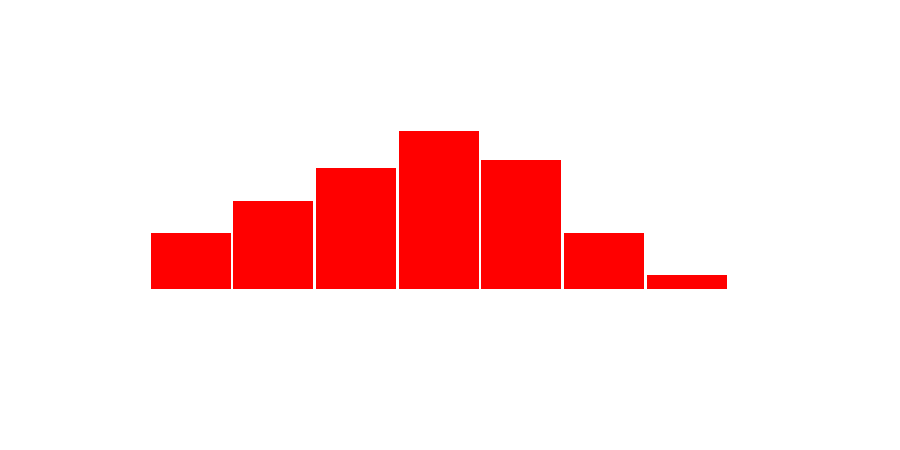
\includegraphics[scale = 0.1, clip = true, trim= 50px 60px 50px 60px]{hist-29b6fa715eecc1dad108c8148465533b.pdf} \\ 
  mergetime\_minutes & Minutes between opening and merging (only for merged pull
    requests) & 0.00 & 10,506 & 418.00 & 44,234 & 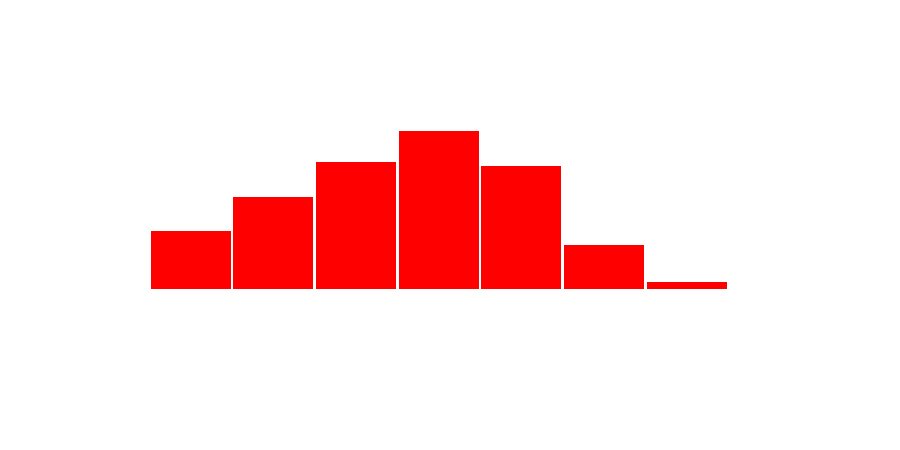
\includegraphics[scale = 0.1, clip = true, trim= 50px 60px 50px 60px]{hist-e2ded77f4080f561e112a1f363b125ce.pdf} \\ 
  num\_commits & Number of commits & 1.00 & 4.42 & 1.00 & 12.00 & 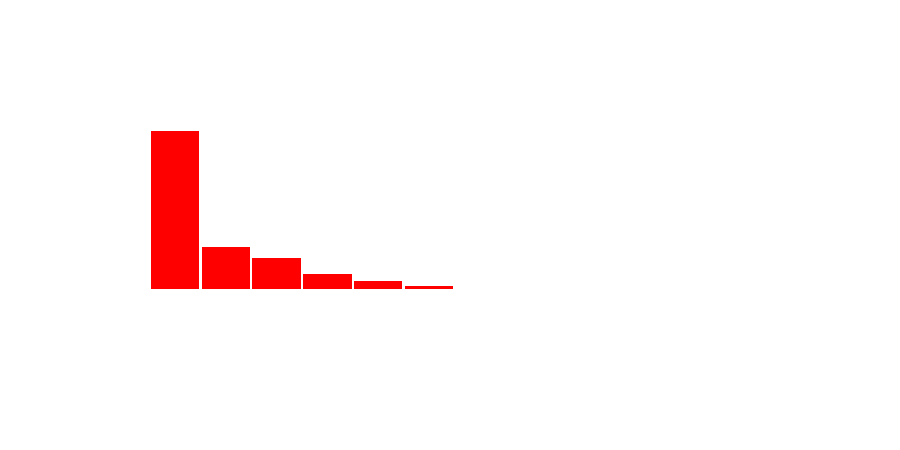
\includegraphics[scale = 0.1, clip = true, trim= 50px 60px 50px 60px]{hist-f128f3cb38588fe5202716588c047381.pdf} \\ 
  src\_churn & Number of lines changed (added + deleted) & 0.00 & 282.95 & 10.00 & 846.00 & 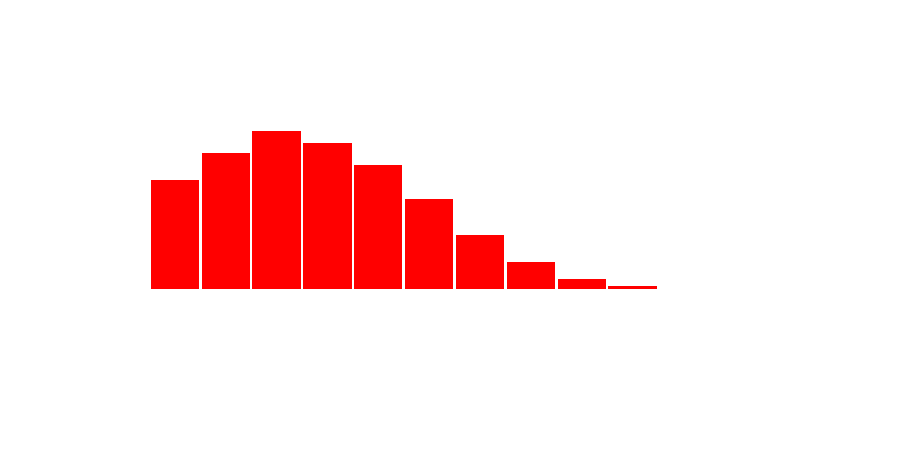
\includegraphics[scale = 0.1, clip = true, trim= 50px 60px 50px 60px]{hist-1f006c80a0da61518435a0c55f538326.pdf} \\ 
  test\_churn & Number of test lines changed & 0.00 & 79.74 & 0.00 & 248.00 & 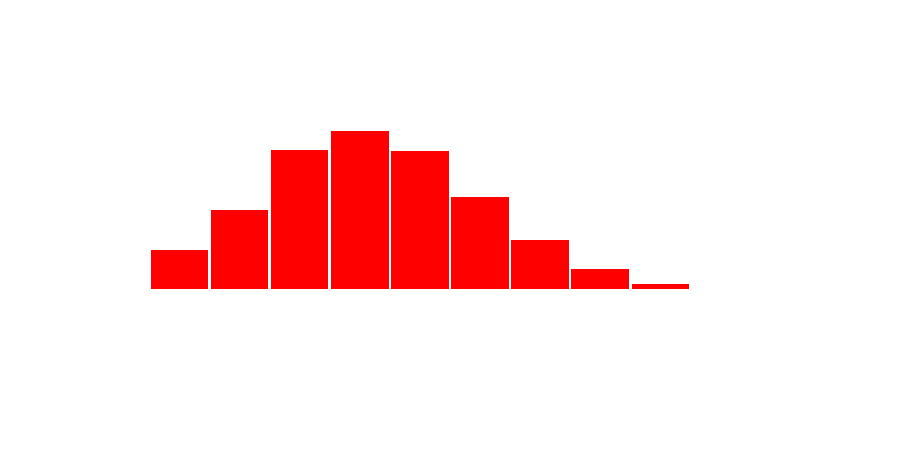
\includegraphics[scale = 0.1, clip = true, trim= 50px 60px 50px 60px]{hist-dd78ccaeedd7fc79735a66eb7f9e506b.pdf} \\ 
  files\_added & Number of files added  & 0.00 & 4.01 & 0.00 & 7.00 & 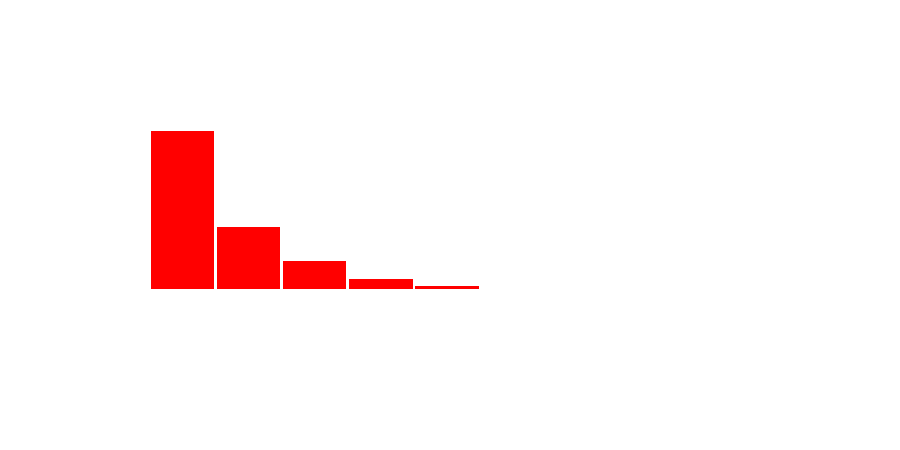
\includegraphics[scale = 0.1, clip = true, trim= 50px 60px 50px 60px]{hist-340be33adc9a51666460c68028842c1d.pdf} \\ 
  files\_deleted & Number of files deleted  & 0.00 & 2.05 & 0.00 & 1.00 & \includegraphics[scale = 0.1, clip = true, trim= 50px 60px 50px 60px]{hist-bd564691a0c6275ea5f30bcc0b81b3f5.pdf} \\ 
  files\_modified & Number of files modified  & 1.00 & 7.56 & 2.00 & 21.00 & 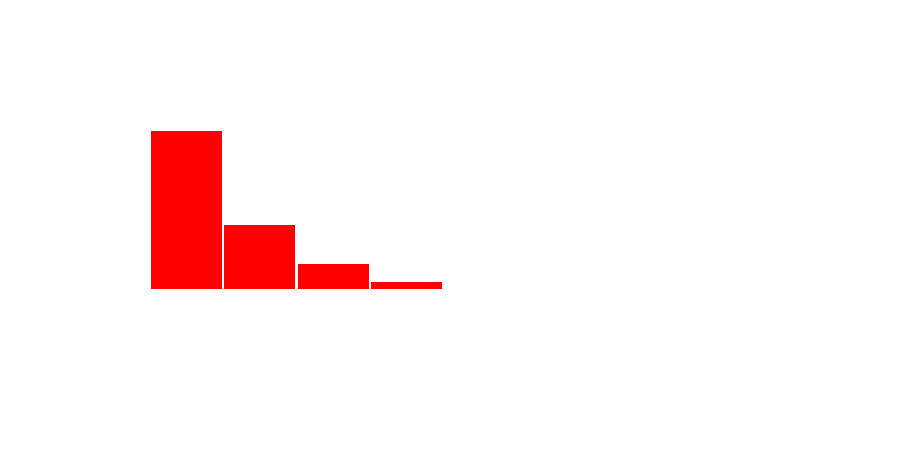
\includegraphics[scale = 0.1, clip = true, trim= 50px 60px 50px 60px]{hist-52a19dc5ca5e4f8c5325bca43137a6c1.pdf} \\ 
  files\_changed & Number of files touched (sum of the above) & 1.00 & 13.62 & 2.00 & 32.00 & 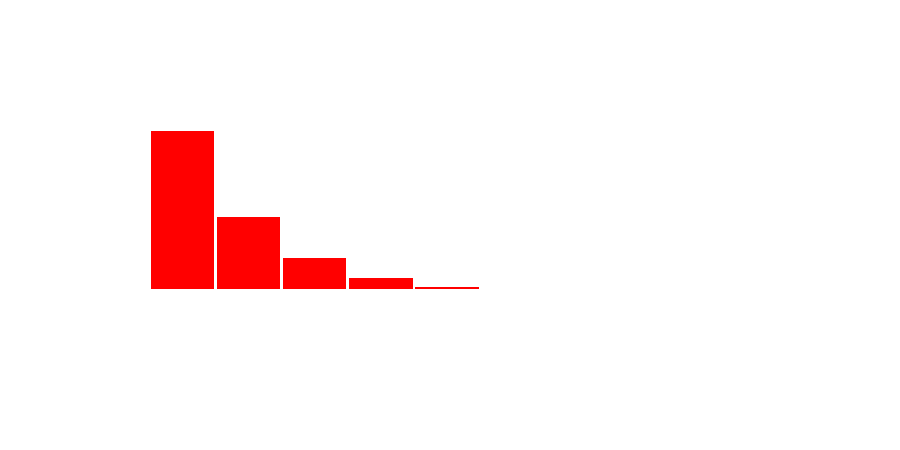
\includegraphics[scale = 0.1, clip = true, trim= 50px 60px 50px 60px]{hist-9b07b060359435635ff2bf4cd34f834a.pdf} \\ 
  src\_files & Number of source code files touched by the pull request & 0.00 & 7.64 & 1.00 & 20.00 & 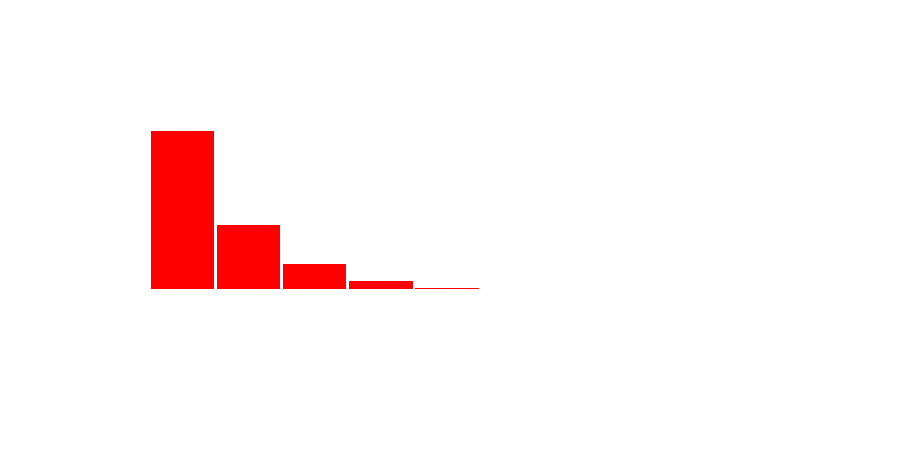
\includegraphics[scale = 0.1, clip = true, trim= 50px 60px 50px 60px]{hist-2d4e53ba8eec29c0c79c1e834756c654.pdf} \\ 
  doc\_files & Number of documentation (markup) files touched & 0.00 & 2.36 & 0.00 & 6.00 & 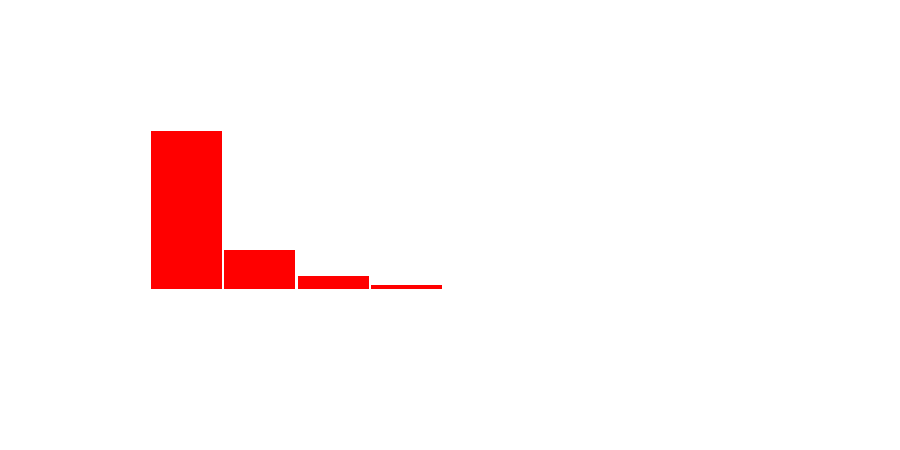
\includegraphics[scale = 0.1, clip = true, trim= 50px 60px 50px 60px]{hist-d4fb585969e7acb86dd568d80e7f1500.pdf} \\ 
  other\_files & Number of non-source, non-documentation files touched & 0.00 & 2.74 & 0.00 & 4.00 & 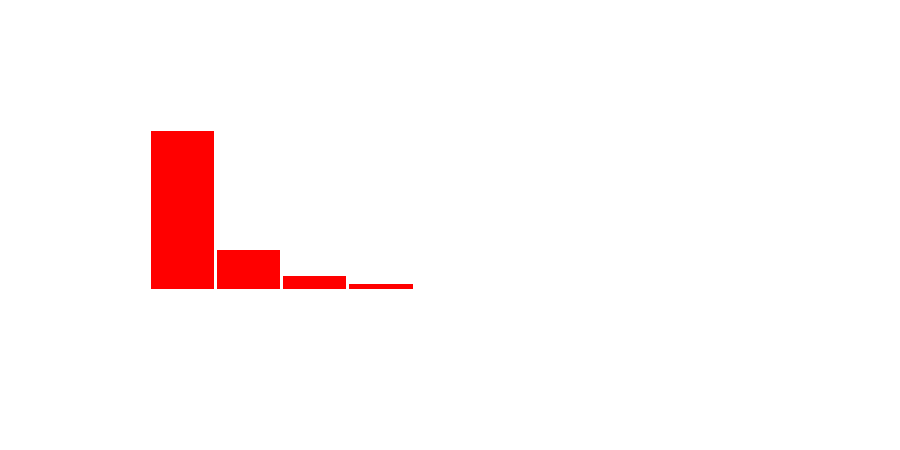
\includegraphics[scale = 0.1, clip = true, trim= 50px 60px 50px 60px]{hist-df965fcd0b03a96f1b31b2eda13d2b98.pdf} \\ 
  num\_commit\_comments & The total number of code review comments & 0.00 & 0.73 & 0.00 & 4.00 & 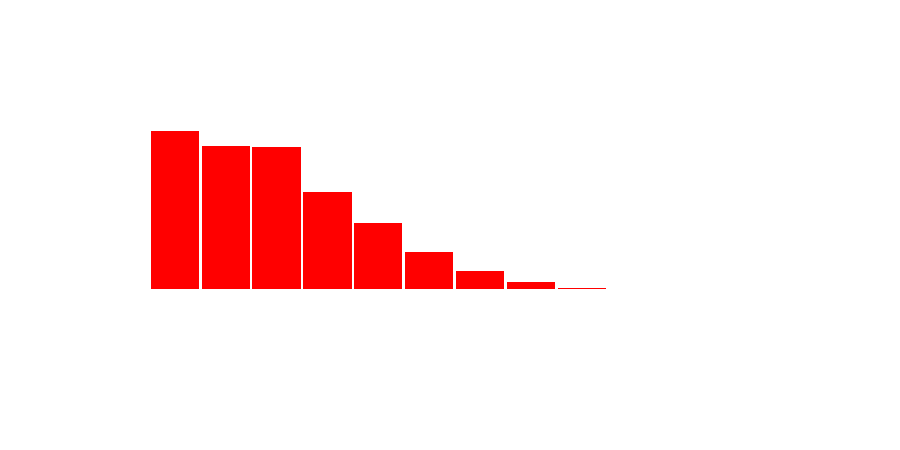
\includegraphics[scale = 0.1, clip = true, trim= 50px 60px 50px 60px]{hist-f0fac61db5a83629be8f04cc84e8b907.pdf} \\ 
  num\_issue\_comments & The total number of discussion comments & 0.00 & 1.84 & 0.00 & 8.00 & 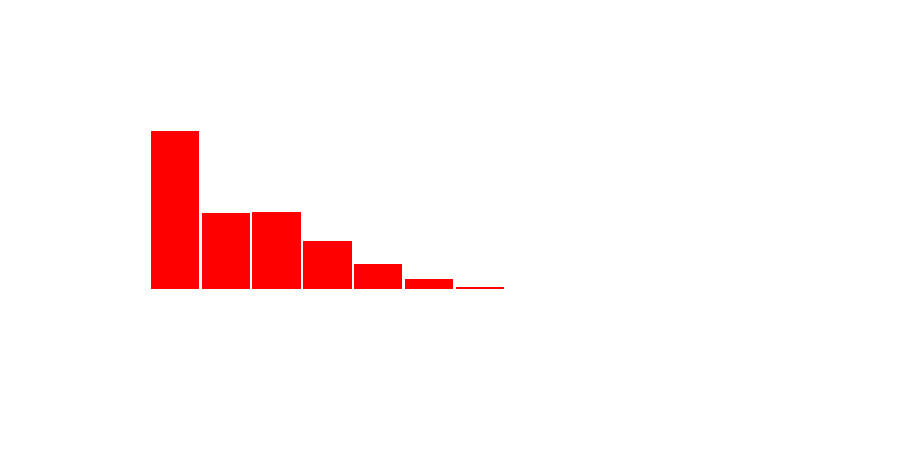
\includegraphics[scale = 0.1, clip = true, trim= 50px 60px 50px 60px]{hist-fee6653ed7b2359f7e7374841378492b.pdf} \\ 
  num\_comments & The total number of comments (discussion and code review). & 0.00 & 2.57 & 1.00 & 11.00 & 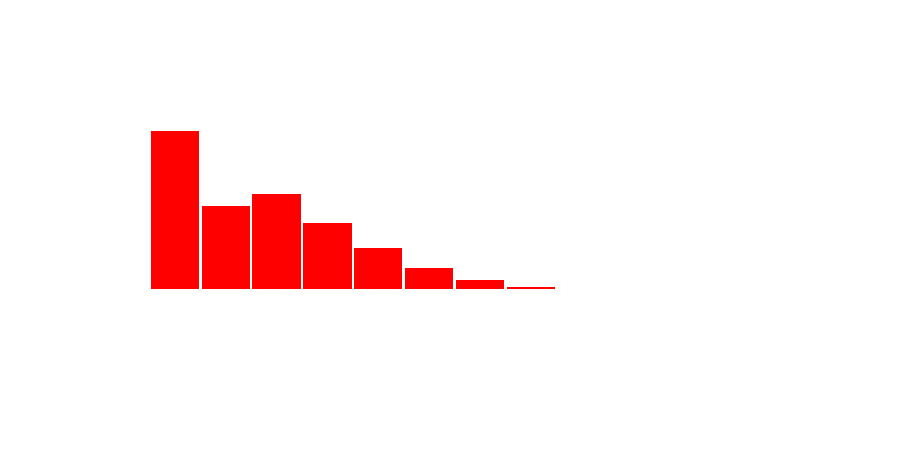
\includegraphics[scale = 0.1, clip = true, trim= 50px 60px 50px 60px]{hist-9db5e2b390de0d64d26c14798cb579ef.pdf} \\ 
  num\_participants & Number of participants in the discussion & 0.00 & 1.27 & 1.00 & 4.00 & 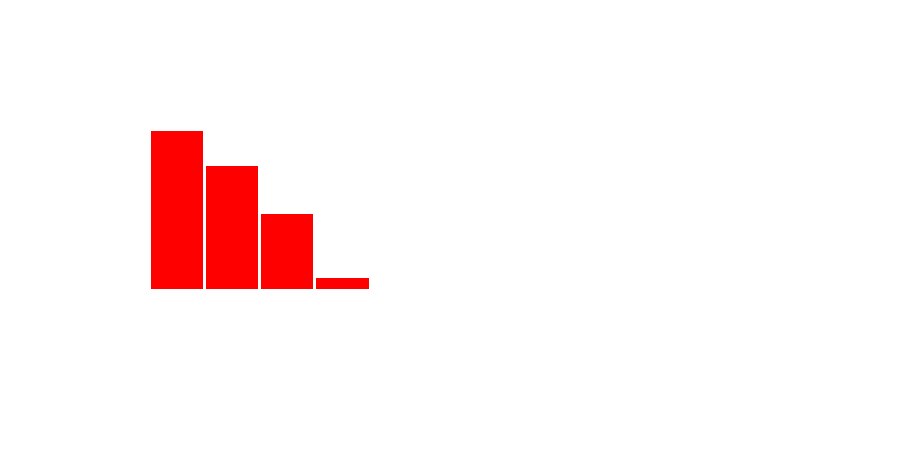
\includegraphics[scale = 0.1, clip = true, trim= 50px 60px 50px 60px]{hist-7d419bb69f175ea7015a9bdc71172f38.pdf} \\ 
  \multicolumn{2}{l}{\bf{Project Characteristics}}\\
  
  sloc & Executable lines of code at creation time. & 458.00 & 53,801 & 18,019 & 275,058 & 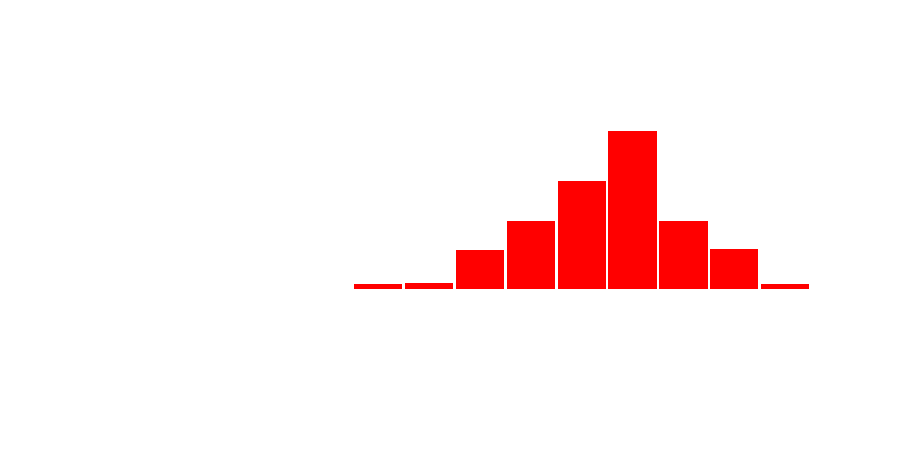
\includegraphics[scale = 0.1, clip = true, trim= 50px 60px 50px 60px]{hist-6b5159d3060b4fdf8493d4c818f79949.pdf} \\ 
  team\_size & Number of active core team members during the last 3 months prior to creation. & 1.00 & 20.64 & 7.00 & 93.00 & 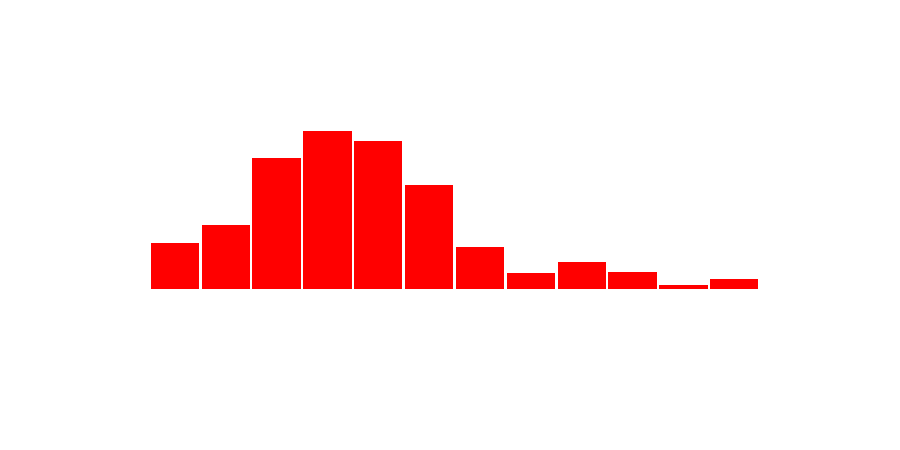
\includegraphics[scale = 0.1, clip = true, trim= 50px 60px 50px 60px]{hist-231fb4fabf4a3f0c551f2a97ae080508.pdf} \\ 
  perc\_external\_contribs & The ratio of commits from external members over core team members in the last 3 months prior to creation. & 8.00 & 54.01 & 56.00 & 95.00 & 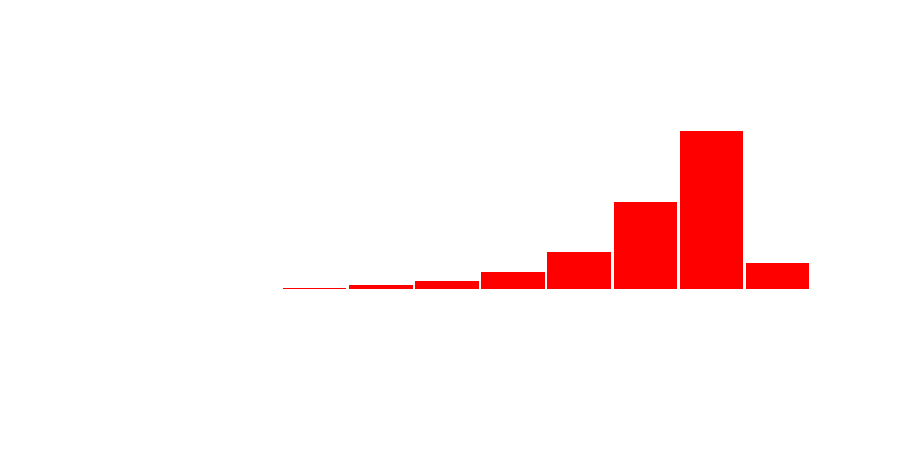
\includegraphics[scale = 0.1, clip = true, trim= 50px 60px 50px 60px]{hist-a222f0a5c377ba129dd6c8f257062591.pdf} \\ 
  commits\_on\_files\_touched & Number of total commits on files touched by the pull request 3 months before the creation time. & 0.00 & 51.65 & 4.00 & 209.00 & 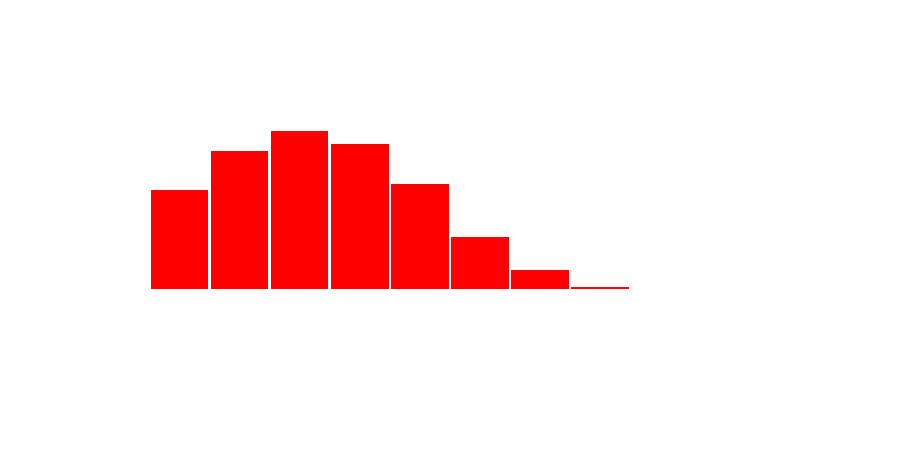
\includegraphics[scale = 0.1, clip = true, trim= 50px 60px 50px 60px]{hist-b735900ffcc37e7eda16dcd0c3497e6e.pdf} \\ 
  test\_lines\_per\_kloc & Executable lines of test code per 1,000 lines of source code & 0.00 & 1,297 & 355.21 & 2,097 & 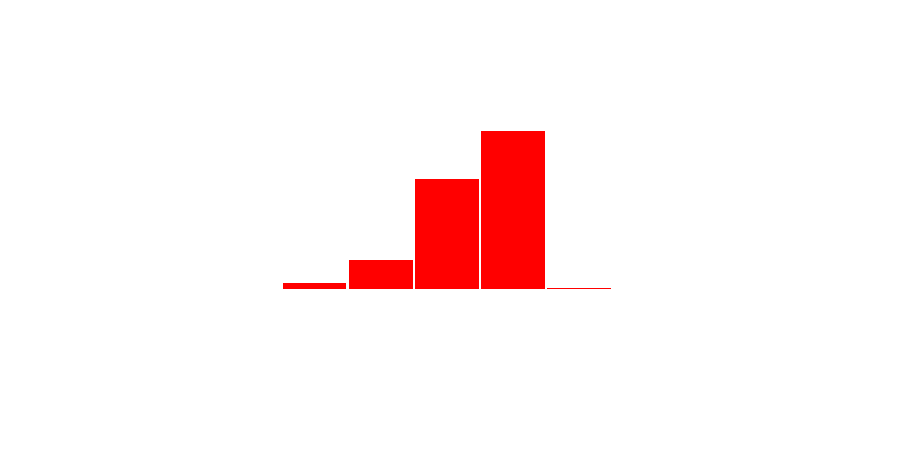
\includegraphics[scale = 0.1, clip = true, trim= 50px 60px 50px 60px]{hist-67ff3047089ba9ce0528884eab66e80a.pdf} \\ 
  test\_cases\_per\_kloc & Number of test cases per 1,000 lines of source code & 0.00 & 83.74 & 14.55 & 181.03 & 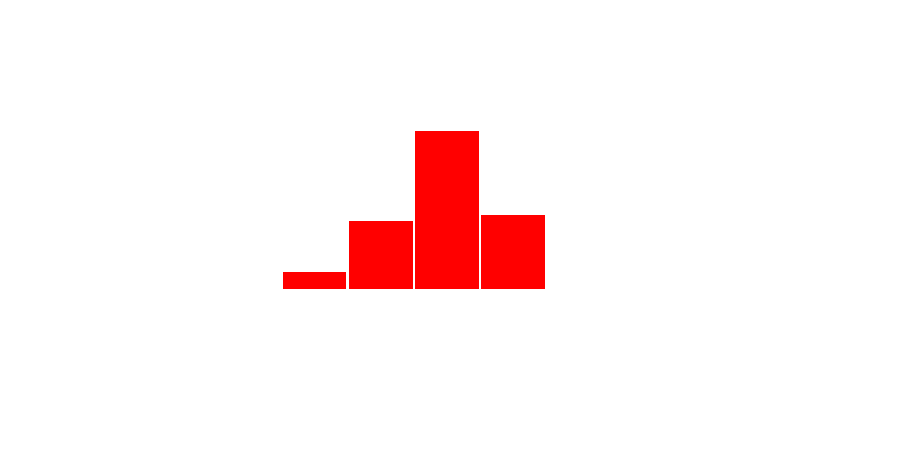
\includegraphics[scale = 0.1, clip = true, trim= 50px 60px 50px 60px]{hist-2b62bb5f7ccb31fe66208a895c8dd549.pdf} \\ 
  asserts\_per\_kloc & Number of assert statements per 1,000 lines of source code & 0.00 & 200.30 & 40.37 & 479.11 & 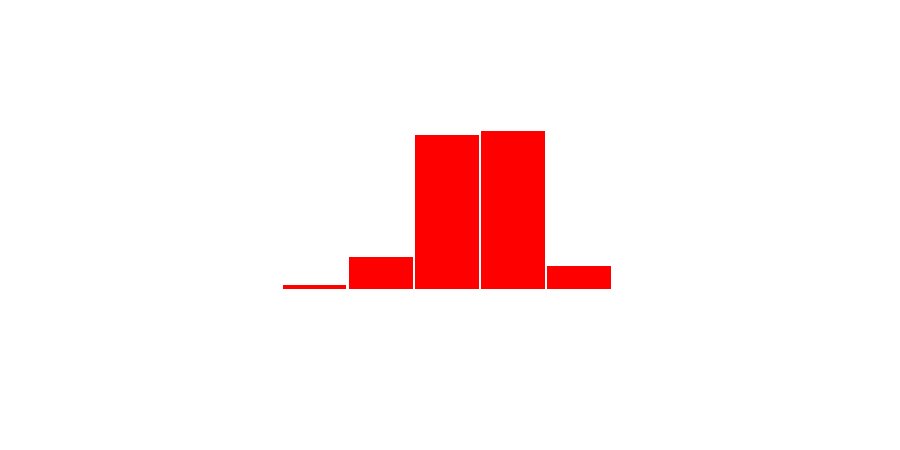
\includegraphics[scale = 0.1, clip = true, trim= 50px 60px 50px 60px]{hist-4ad84a89acf32483001ce11c881622b8.pdf} \\ 
  watchers & Project watchers (stars) at creation & 4.00 & 1,778 & 310.00 & 11,114 & 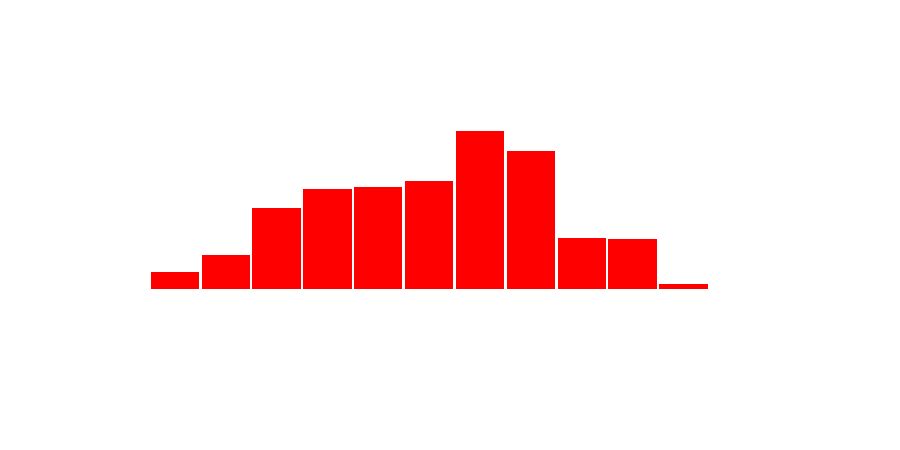
\includegraphics[scale = 0.1, clip = true, trim= 50px 60px 50px 60px]{hist-d097a7d1786ca9917e46e0fda1adb365.pdf} \\

  \multicolumn{2}{l}{\bf{Developer Characteristics}}\\
  
  prev\_pullreqs & Number of pull requests submitted by a specific developer, prior to the examined one & 0.00 & 42.81 & 11.00 & 196.00 & 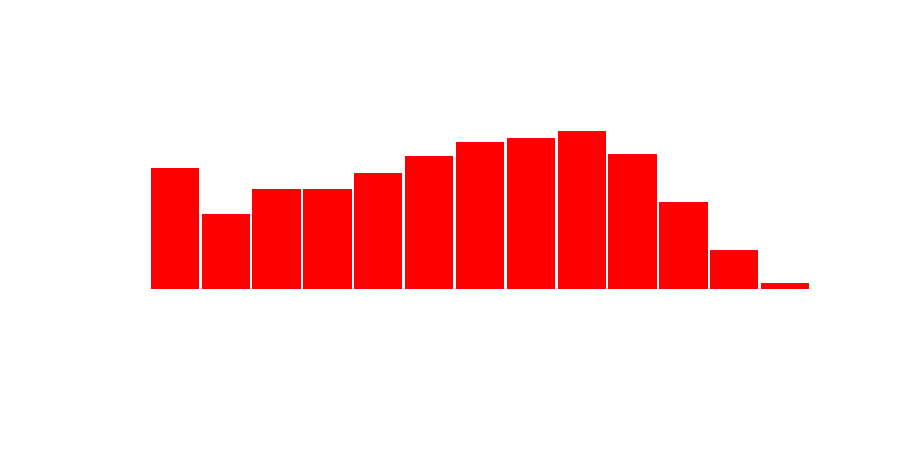
\includegraphics[scale = 0.1, clip = true, trim= 50px 60px 50px 60px]{hist-a2f7f60851dfa13cfbe0227d1d233767.pdf} \\ 
  requester\_succ\_rate & The percentage of the developer's pull requests that have been merged up to the creation of the examined one & 0.00 & 0.51 & 0.62 & 1.00 & 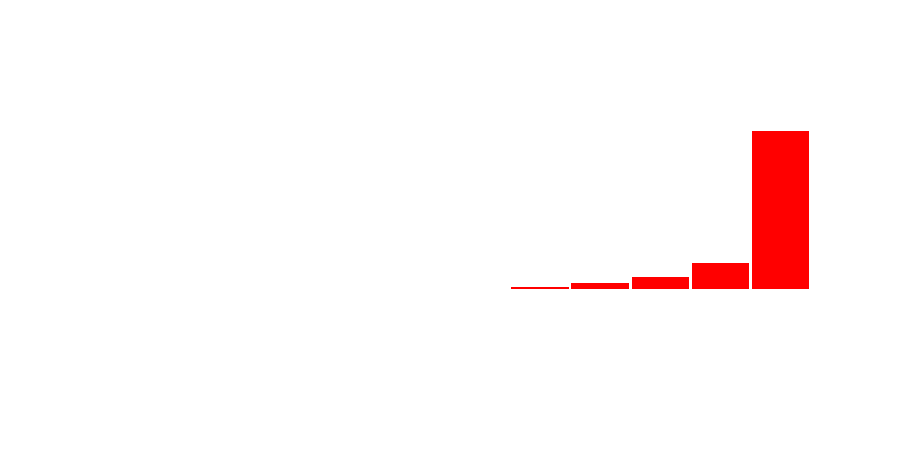
\includegraphics[scale = 0.1, clip = true, trim= 50px 60px 50px 60px]{hist-9363017165c3ded62457750f1c67c1af.pdf} \\ 
  followers & Followers to the developer at creation & 0.00 & 20.93 & 4.00 & 80.00 & 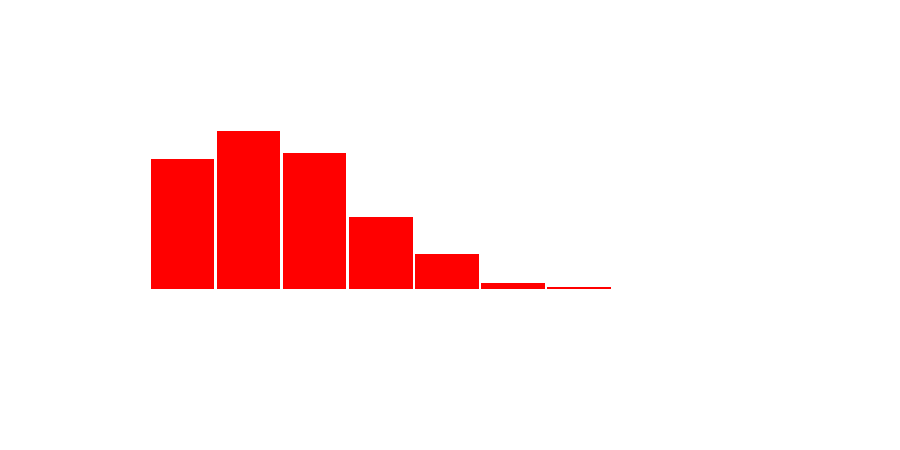
\includegraphics[scale = 0.1, clip = true, trim= 50px 60px 50px 60px]{hist-a7f2f738f15a09420e70e9a2c30e2aef.pdf} \\ 
   \hline
\end{tabular}
\caption{Selected features and descriptive statistics. A data point is a pull request. Historgrams are in log scale.} 
\label{tab:features}
\end{table*}


%\begin{figure}
%  \begin{center}
%    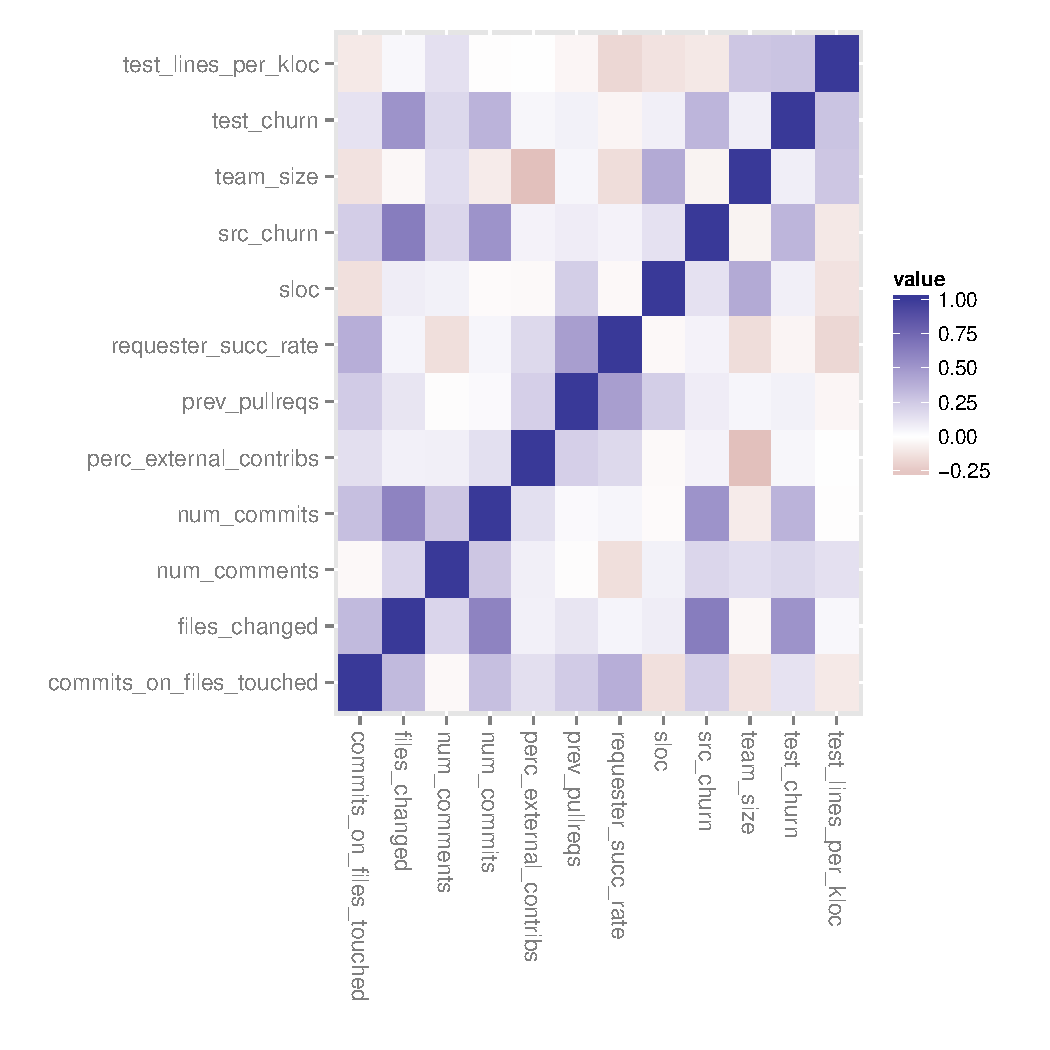
\includegraphics[scale=0.5]{cross-cor-heat.pdf}
%  \end{center}
%  \caption{Cross correlation heat map (Spearman) for selected features.}
%  \label{fig:crosscor}
%\end{figure}

\vspace{1em}
\subsection{Qualitative data}
\label{sec:qualdata}
To investigate how pull requests are used in practice and why some pull requests
are not merged, we performed in-depth examination of random samples of pull
requests followed by coding and thematic analysis. 100 pull requests were initially
used by the first coder to identify discrete reasons for closing pull requests
(bootstrapping sample), while a different set of 100 pull requests were used by
all three coders to validate the identified categories (cross-validation
sample). After cross validation, the two datasets were merged and a further 150 randomly selected pull requests
were added to the bootstrapping sample to construct the finally analyzed
dataset for a total of 350 pull requests.

%To examine how pull requests are used in practice, we categorized
%100 randomly selected pull requests, sampled from the dataset described above,
%in two categories: patches and feature discussions. We drew those categories
%from our experience as pull request users and also by consulting 
%the interviews in Pham et al.~\cite{Pham13} and Marlow et al.~\cite{Marlo13}.

\section{Popularity of Pull-based Development}
\label{sec:github}
%% latex table generated in R 2.15.3 by xtable 1.7-1 package
% Fri Sep  6 17:15:25 2013
\begin{table*}[ht]
\centering
\begin{tabular}{rccccccc}
  \hline
description & min & quant\_5 & median & mean & quant\_95 & max & histogram \\ 
  \hline
Number of participants & 0.00 & 0.00 & 1.00 & 1.39 & 3.00 & 91.00 & 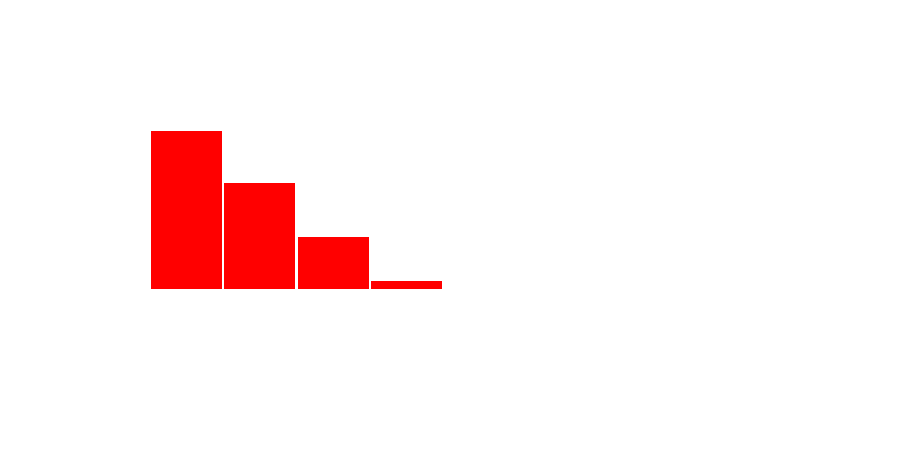
\includegraphics[scale = 0.1, clip = true, trim= 50px 60px 50px 60px]{hist-c83eb37a528ffcd758150a237ae378c7.pdf} \\ 
  Number of comments & 0.00 & 0.00 & 0.00 & 1.70 & 7.00 & 642.00 & 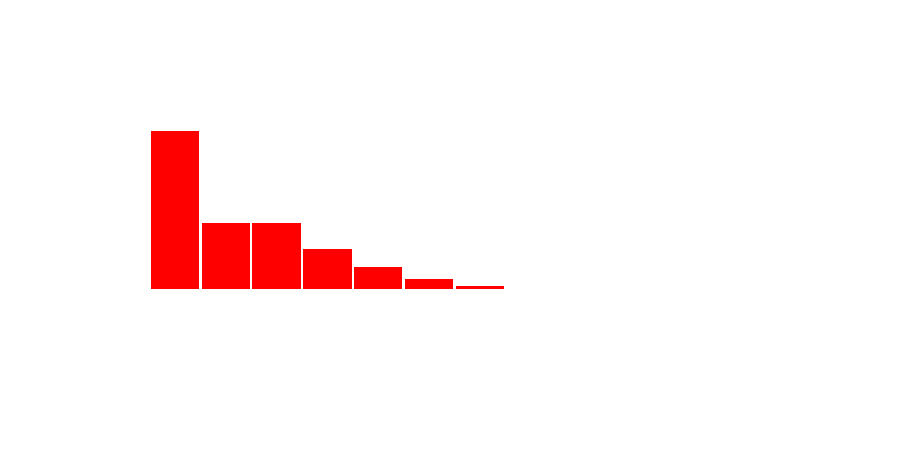
\includegraphics[scale = 0.1, clip = true, trim= 50px 60px 50px 60px]{hist-0d7111a5679c9d7ae097710bfbe5ad46.pdf} \\ 
  Number of commits & 1.00 & 1.00 & 1.00 & 5.00 & 14.00 & 1745.00 & 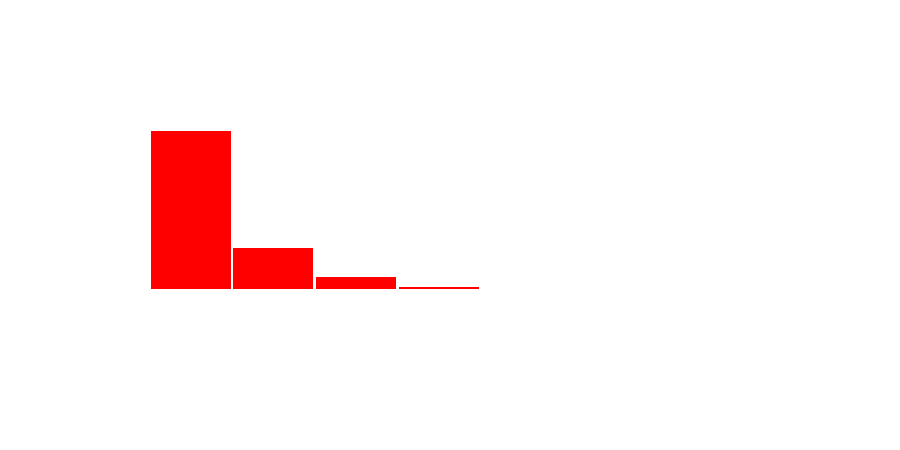
\includegraphics[scale = 0.1, clip = true, trim= 50px 60px 50px 60px]{hist-a86184e179390a51b3bf0b4a000ff1bf.pdf} \\ 
  Time to merge (min) & 0.00 & 0.00 & 157.00 & 7315.10 & 28883.30 & 1493913.00 & 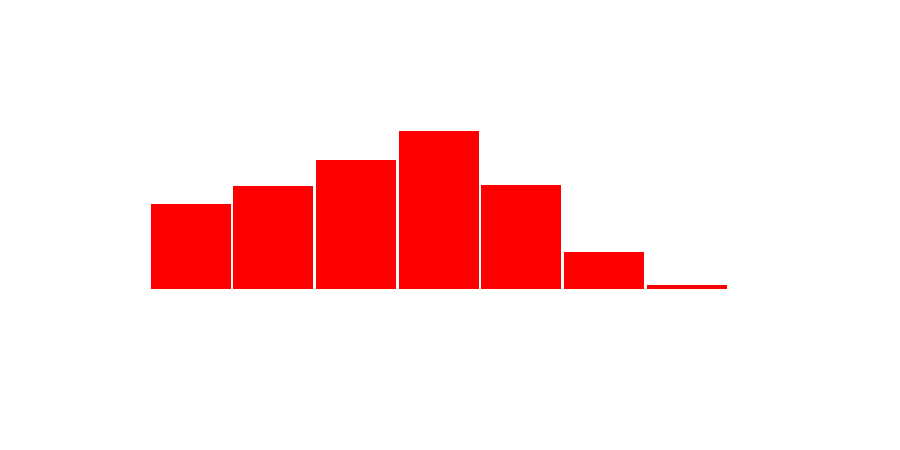
\includegraphics[scale = 0.1, clip = true, trim= 50px 60px 50px 60px]{hist-d5b282b6f57817578bf430989f92d122.pdf} \\ 
  Time to close (min) & 0.00 & 0.00 & 1108.00 & 30302.73 & 172754.95 & 1556363.00 & 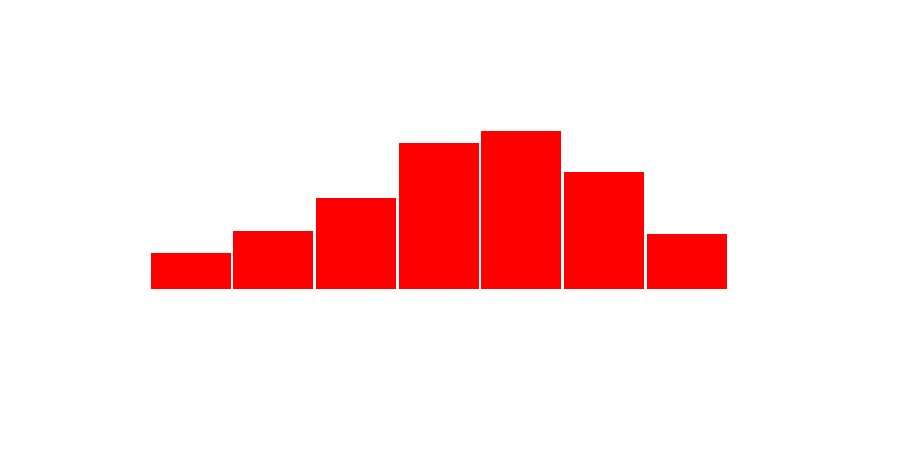
\includegraphics[scale = 0.1, clip = true, trim= 50px 60px 50px 60px]{hist-b2793dce9a27260faa7c8b85aeb789d2.pdf} \\ 
   \hline
\end{tabular}
\caption{Descriptive statistics for pull requests across all projects in the GHTorrent dataset (1.8M). Historgrams are in log scale.} 
\label{tab.overall.stats}
\end{table*}


%\begin{figure}[t]
%  \centering
%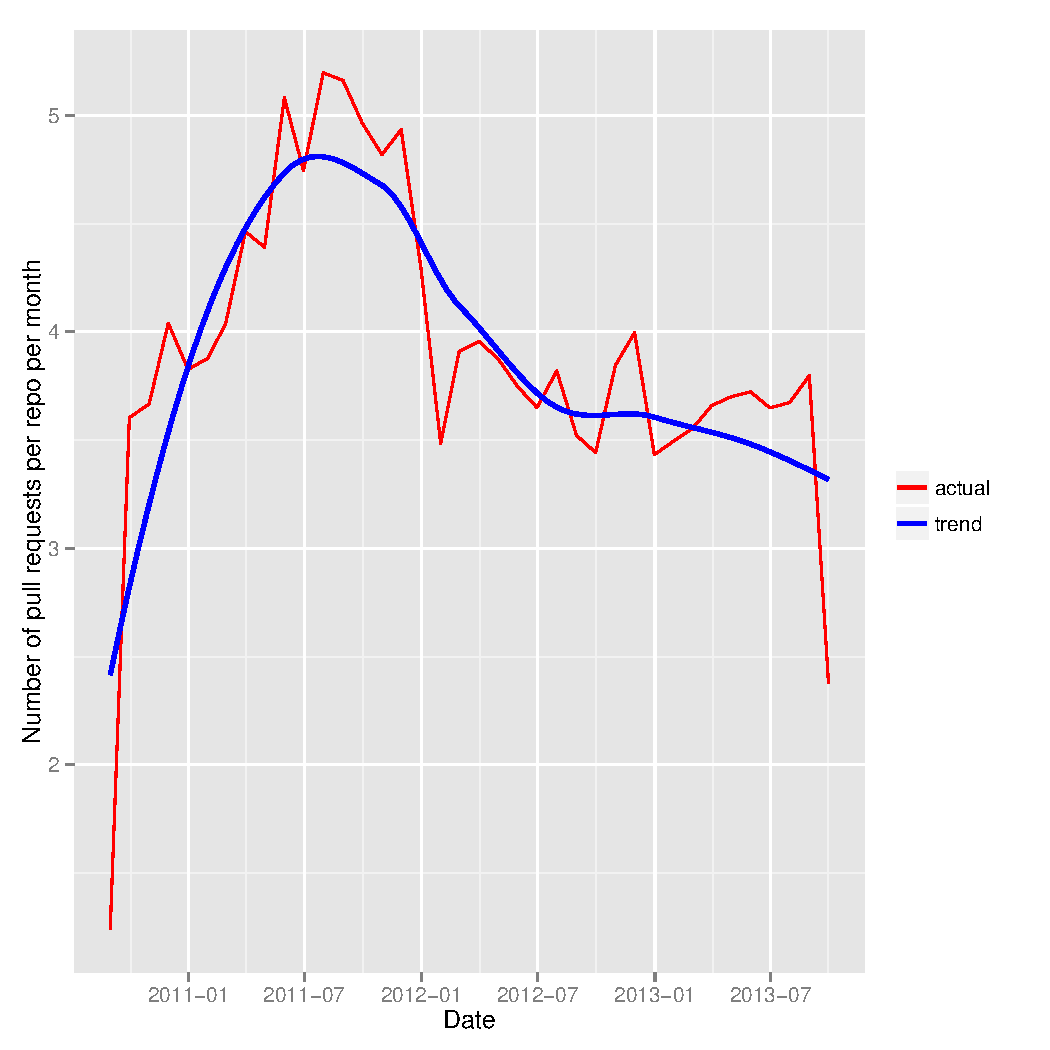
\includegraphics[scale=0.45]{num-pullreqs-month.pdf}
%\label{fig:num-pullreqs-month}
%\caption{Number of pull requests per repo per month on all Github repositories.}
%\end{figure}

As of August 2013, Github reports
more than 7 million repositories and 4 million users. However, not all those
projects are active: in the period Feb 2012 --- Aug 2013, the {\sc ght}orrent dataset captured events initiated by
(approximately) 2,281,000 users affecting 4,887,500 repositories. The majority
of registered repositories are forks of other repositories, special repositories
hosting user web pages 
%(named as \texttt{<name>.github.com}),
program
configuration files 
%(\texttt{dotfiles}) 
and temporary repositories for evaluating Git. 
%(\texttt{try\_git}). 
In the {\sc ght}orrent dataset, less than half
(1,877,660 or 45\%) of the active repositories are original repositories.

Pull requests are enabled by default on all repositories opened on Github;
however, not all projects are using them to collaborate.  In the period from
February to August 2012, 315,522 original repositories received a single commit.
From those, 53,866 (17\%) received at least one pull request, while 54,205
(18\%) used the shared repository approach, having received commits by more than
one developers and no pull requests.  The situation is similar during the same
period in 2013; from the 1,157,625 repositories that received a single commit,
120,104 (10\%) repositories received a pull request while 124,316 (11\%) used
the shared repository approach exclusively. Across both years, 14\% of the
active repositories use pull requests.  While pull request usage is increasing
overall, partially reflecting Github's growth, the relative number of
repositories using the pull request model has decreased slightly.  An almost
equal number of projects use pull requests and shared repositories for
distributed collaboration.

%On a per repository basis, the average number of pull requests per month is stable
%between 2012 and 2013, as we see in Figure~\ref{fig:num-pullreqs-month}.
For those projects that received pull requests in 2013, the mean number of pull
requests per project is relatively low at 8.1 (median: 2, percentiles: 5\%: 1,
95\%: 21); however, the distribution of the number of pull requests in projects
is highly skewed. Projects exists, such as Ruby on Rails and the Homebrew
package manager, that have more that 5,000 pull requests. From the pull requests
that have been opened in 2013, 73,07\% have been merged using Github facilities,
thereby indicating that pull requests in principle can work as a means for
obtaining external contributions. Moreover, even though one might expect that it
is the well known projects that receive most pull requests, this is only
moderately supported by our data: the Spearman rank correlation between the
number of stars of a project and the number of pull requests it has received is
$\rho = 0.36$ ($p < 0.001, n = 239,131$).

Reviews on a pull request can either target the pull as whole or the individual
commits, thereby resembling a code review. On average, each pull request
receives 2,89 (quantiles: 5\%: 0, 95\%: 11, median: 1) discussion and code
review comments.  Even though any Github user can participate in the review
process, usually it is the project community members that do so: only 0.011\% of
pull request comments come from users that have not committed to the project
repository. Across projects that received pull requests in 2012, 35\% also
received a bug report (not pull-request based) on the Github issue tracker,
indicating a strong use of Github's collaboration facilities by both the project
and the project community.

%Pull requests in their current form were introduced by Github in late August
%2010. As can be seen in Figure~\ref{fig:before-after-pr}, on certain long lived
%projects, the introduction of pull requests had significantly increased the
%number of contributors per month. To investigate whether the introduction of
%pull requests had a measurable effect on projects that used them, we calculated
%the mean number of active developers per month for a period of 12 months before
%and after the introduction of pull requests. We filtered out projects that begun
%using pull requests only after September 2011 and those whose average number of
%developers is less than two (indicating self-submission and acceptance of pull
%requests). We performed a paired Mann-Whitney test across the means for each
%project, which indicated a statistically significant difference ($n = 362, V =
%56690, p < 0.001$). We also calculated the effect size using Cliff's $\delta =
%0.42$. This indicates a statistically significant increase in the mean number of
%developers per month after the introduction of pull requests, even though this
%does not necessarily mean that pull requests are indeed the reason.
%
%\begin{figure}
%  \begin{center}
%    
\includegraphics[scale=0.5]{num-commiters-after-pr}
%  \end{center}
%  \caption{Number of committers before and after the introduction of pull
%  requests by Github. The lines are smoothed using the local polynomial
%  regression fitting method, to account for monthly fluctuations.}
%  \label{fig:before-after-pr}
%\end{figure}


\noindent
\fbox{
\begin{minipage}{0.46\textwidth}
\emph{RQ1: 14\% of repositories are using pull requests on Github.
Pull requests and shared repositories are equally used among projects.
Pull request usage is increasing in absolute numbers, even though the proportion of repositories using pull requests has decreased slightly.}
\end{minipage}}
%

%% latex table generated in R 2.15.3 by xtable 1.7-1 package
% Fri Aug 23 15:19:16 2013
\begin{table}[ht]
\centering
{\small
\begin{tabular}{rrrrrrrrrrrrr}
  \hline
 & team\_size & num\_commits & files\_changed & perc\_external\_contribs & sloc & src\_churn & test\_churn & commits\_on\_files\_touched & test\_lines\_per\_kloc & prev\_pullreqs & requester\_succ\_rate & num\_comments \\ 
  \hline
team\_size & 1.00 & -0.09 & -0.03 & -0.28 & 0.41 & -0.04 & 0.08 & -0.15 & 0.26 & 0.03 & -0.19 & 0.16 \\ 
  num\_commits & -0.09 & 1.00 & 0.57 & 0.14 & -0.00 & 0.50 & 0.32 & 0.28 & -0.02 & 0.02 & 0.04 & 0.26 \\ 
  files\_changed & -0.03 & 0.57 & 1.00 & 0.06 & 0.09 & 0.62 & 0.49 & 0.30 & 0.03 & 0.12 & 0.06 & 0.17 \\ 
  perc\_external\_contribs & -0.28 & 0.14 & 0.06 & 1.00 & -0.03 & 0.05 & 0.04 & 0.15 & 0.01 & 0.22 & 0.13 & 0.11 \\ 
  sloc & 0.41 & -0.00 & 0.09 & -0.03 & 1.00 & 0.16 & 0.06 & -0.14 & -0.15 & 0.21 & -0.02 & 0.04 \\ 
  src\_churn & -0.04 & 0.50 & 0.62 & 0.05 & 0.16 & 1.00 & 0.33 & 0.21 & -0.11 & 0.09 & 0.07 & 0.18 \\ 
  test\_churn & 0.08 & 0.32 & 0.49 & 0.04 & 0.06 & 0.33 & 1.00 & 0.12 & 0.31 & 0.06 & -0.02 & 0.16 \\ 
  commits\_on\_files\_touched & -0.15 & 0.28 & 0.30 & 0.15 & -0.14 & 0.21 & 0.12 & 1.00 & -0.08 & 0.25 & 0.34 & -0.00 \\ 
  test\_lines\_per\_kloc & 0.26 & -0.02 & 0.03 & 0.01 & -0.15 & -0.11 & 0.31 & -0.08 & 1.00 & -0.03 & -0.12 & 0.14 \\ 
  prev\_pullreqs & 0.03 & 0.02 & 0.12 & 0.22 & 0.21 & 0.09 & 0.06 & 0.25 & -0.03 & 1.00 & 0.47 & -0.02 \\ 
  requester\_succ\_rate & -0.19 & 0.04 & 0.06 & 0.13 & -0.02 & 0.07 & -0.02 & 0.34 & -0.12 & 0.47 & 1.00 & -0.10 \\ 
  num\_comments & 0.16 & 0.26 & 0.17 & 0.11 & 0.04 & 0.18 & 0.16 & -0.00 & 0.14 & -0.02 & -0.10 & 1.00 \\ 
   \hline
\end{tabular}
}
\caption{Cross correlation matrix (Spearman) between examined factors} 
\label{tab:crosscor}
\end{table}


\section{Pull Request Lifecycle}
\label{sec:pullreqchar}

\textbf{Lifetime of pull requests.}
After being submitted, pull requests can be in two states: merged or closed
(and therefore not-merged).
In our dataset, most pull requests (84.73\%) are eventually
merged. This result is higher than the overall we calculated for
Github; we attribute this to the fact that the dataset generation
process employs heuristics to detect merges in addition to those happening
with Github facilities.

For merged pull requests, an important property is the time required to process
and merge them. The time to merge distribution is highly skewed, with the great
majority of merges happening very fast. Measured in days, 95\% of the pull
requests are merged in 26, 90\% in 10 and 80\% in 3.7 days. 30\% of pull
requests are merged in under one hour; the majority of such pull requests (60\%)
come from the community, while their source code churn is significantly lower
than that of the pull requests from the main team members (medians: 5 and 13
lines respectively). If we compare the time to process pull requests that are being
merged against those that are not, we can see that pull requests that have been
merged are closed much faster (median: 434 minutes) than unmerged (median: 2,250
minutes) pull requests.  The results of an unpaired Mann-Whitney test ($p <
0.001$) showed that this difference is statistically significant, with a
moderately significant effect size (Cliff's $\delta: 0.32$). This means that
pull requests are either processed fast or left lingering for long before they
are closed.

Based on these observations, we check whether the pull
requests originating from main team members are treated faster than those from
external contributors. To answer it, we performed an unpaired Mann-Whitney test
among the times to merge pull requests from each group. The result is that while
the two groups differ in a statistically significant manner ($n_1 = 51,829, n_2
= 89,454, p < 0.001$), the apparent difference is negligible (Cliff's $\delta:
-0.09$). This means that merged pull requests received no special treatment,
irrespective whether they came from core team members or from the community.

On a per project basis, if we calculate the median time to merge a pull request,
we see that in the vast majority of projects (97\%), the median time to merge a
pull request is less than 7 days. The mean time to merge is not correlated with
the project's size ($\rho = -0.05$), nor the project's test coverage ($\rho =
0.27$). It is however, strongly correlated ($\rho = -0.69$) with the
contributor's track record: the more pull requests a developer has submitted to
the same project, the lower the time to process each one of them.  Moreover,
projects are not getting faster at pull request processing by processing more
pull requests; the correlation between the mean time to merge and the number of
pull requests the project received is weak ($\rho = -0.23, n = 291, p < 0.01$).

%\fbox{
%\begin{minipage}{0.46\textwidth}
%\emph{80\% of pull requests are merged in less than 3 days, while 30\% are
%merged within one hour. Pull requests are treated the same irrespective of
%their origin (project team or community). The developer's track record
%is an indicator of how fast a pull request will be merged.}
%\end{minipage}}
%
%\begin{figure}
%\centering
%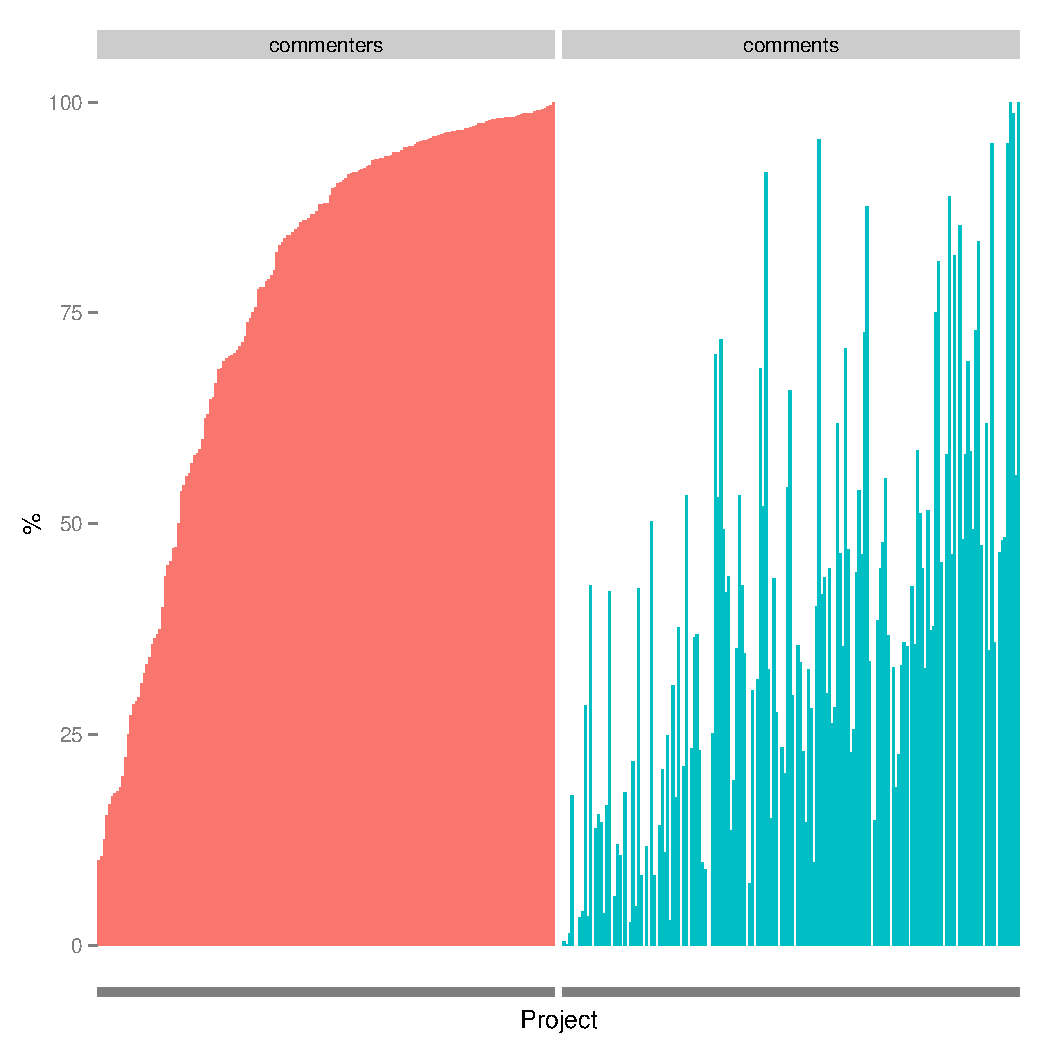
\includegraphics[scale=0.45]{perc-external-commenters-comments.pdf}
%\label{fig:pull-num-comments}
%\caption{Percentage of external commenters and comments per project. Bars
%are sorted by percentage of external commenters. Project names omitted for
%clarity.}
%\end{figure}

\textbf{Sizes of pull requests.}
A pull request bundles together a set of commits; the number of commits on a
pull request is generally less than 10 (95\% percentile: 12, 90\% percentile: 6,
80\% percentile: 3), with a median of 1. The number of files that are changed by
a pull request is generally less than 20 (95\% percentile: 36, 90\% percentile:
17, 80\% percentile: 7), with median number of 2. The number of total lines
changed by pull requests is on average less than 500 (95\% percentile: 1227,
90\% percentile: 497, 80\% percentile: 168) with a median number of 20.

\textbf{Tests and pull requests.} Except from the project's source code, pull
requests also modify test code. In our sample, 33\% of the pull requests
included modifications in test code, while 4\% modified test code exclusively.
Of the pull requests that included modifications to test code, 83\% were merged,
which is similar to the average. This seems to go against the findings by Pham
et al.~\cite{Pham13}, where interviewed developers identified the presence of
tests in pull requests as a major factor for their acceptance. The presence of
tests in a pull request does not seem to affect the merge time either: an
unpaired Mann-Whitney test shows that while there is a statistically significant
difference in the means of the pull request merge time between pull requests
that include tests (median: 17 hours) and those that do not (median: 5 hours)
($pr\_tests = 45,488, pr\_no\_tests = 95,980, p < 0.001$), the effect size is
small ($\delta = 0.18$).

%\fbox{
%\begin{minipage}{0.46\textwidth}
%\emph{Including test code does not help pull requests to be processed faster.}
%\end{minipage}}

\textbf{Discussion and code review.}
Once a pull request has been submitted, it is open for discussion until it is
merged or closed. The discussion is usually brief: 95\% of pull requests receive
12 comments or less (80\% less than 4 comments).
Similarly, the number of participants in the discussion is also low (95\% of
pull requests are discussed by less than 4 people).
The number of
comments in the discussion is moderately correlated with the time to merge a
pull request ($\rho = 0.48, n = 141,468$) and the time to close a non-merged
pull request ($\rho = 0.37, n = 25,416$). 

Code reviews are integrated in the pull request process. While the pull request
discussion can be considered an implicit form of code review, 12\% of the pull
requests in our sample have also been through explicit code reviewing, by having
received comments on source code lines in the included commits. Code reviews do
not seem to increase the probability of a pull request being merged (84\% of
reviewed pull requests are merged), but they do slow down the processing of a
pull request: the unpaired Mann-Whitney test between the time required to merge
reviewed (median: 2719 minutes) and non-reviewed (median: 295 minutes) pull
requests gives statistically significant differences with a significant effect
size ($\delta = 0.41$). Projects that employ code reviews feature larger code
bases and bigger team sizes than those that do not.

Any Github user can participate in the discussion of any pull request. Usually,
the discussion occurs between core team members trying to understand the changes
introduced by the pull request and community members (often, the pull request
creator) who explain it.
In most projects, more than half of the participants are
community members. This is not true however for the number of comments; in most
projects the majority of the comments come from core team members. One might
think that the bigger the percentage of external commenters on pull requests,
the more open the project is and therefore the higher the percentage of
external contributions; a Spearman test indicates that it is not true ($\rho =
0.22, n = 291, p < 0.05$).

\noindent
\fbox{
\begin{minipage}{0.46\textwidth}
  \emph{RQ2: Most pull requests are less than 20 lines long and processed
  (merged or discarded) in less than 1 day. The discussion spans on average to 3
  comments, while code reviews affect the time to merge a pull request.
  Inclusion of test code does not affect the time or the decision to merge a pull request. Pull requests receive no special treatment, irrespective whether they
  come from contributors or the core team.}
\end{minipage}}

\section{Factors influencing merging and merge time}
\label{sec:accrej}

\begin{table}
  \centering
  \begin{tabular}{lcccc}
    \hline
    {\bf classifier} & {\sc auc} & {\sc acc} & {\sc prec} & {\sc rec} \\
    \hline
    \multicolumn{4}{l}{\textsf{mergedecision} task($n = 166,884$)} \\
    binlogregr    & 0.75 & 0.61 & 0.95  & 0.55 \\
    naivebayes    & 0.71 & 0.59 & 0.94 &  0.55 \\
    randomforest  & 0.94 & 0.86 & 0.93 & 0.94 \\
    \hline
    \multicolumn{4}{l}{\textsf{merge time} task($n = 141,468$)} \\
    multinomregr  & 0.61 & 0.44 & --- & --- \\
    naivebayes    & 0.63 & 0.38 & --- & ---  \\
    randomforest  & 0.73 & 0.59 & --- & ---   \\
    \hline
  \end{tabular}
  \caption{Classifier performance for the merge decision and merge time
  classification tasks. The results are means of 10-fold random selection
  cross validation on all data, with 90\% train and 10\% test data.}
  \label{tab:classif-perf}
\end{table}

To understand which factors affect the decision to merge and the time it takes to make this decision,
we run the classification processes according to the method specified in
Section~\ref{sec:resdesign}. Each classifier attempts to predict the dependent
variable (merge decision, merge time class) based on the features presented in
Table~\ref{tab:features}. For the \textsf{mergetime} experiment, we excluded the
\texttt{num\_comments}, \texttt{num\_commits} and \texttt{num\_participants}
features as they could not be measured at the pull request arrival
time. Based on the results presented in Table~\ref{tab:classif-perf}, we
selected the \texttt{randomforest} classification algorithm for both our
experiments. For the \textsf{mergetime} experiment, \texttt{randomforest}
achieved an {\sc auc} of 0.73, with a prior probability of 31\%, 35\% and 34\%
for each of the \textsf{hour}, \textsf{day} and \textsf{more than a day} classes
respectively. For the \textsf{mergedecision} experiment, the prior probability
for the dominant class was 84\% which allowed the algorithm to achieve near
perfect scores. In both cases, the stability of the {\sc auc} metric across
folds was good (\textsf{mergetime}: $\sigma_{auc} = 0.019$,
\textsf{mergedecision}: $\sigma_{auc} = 0.008$).

\begin{figure*}
\centering
\subfigure {
  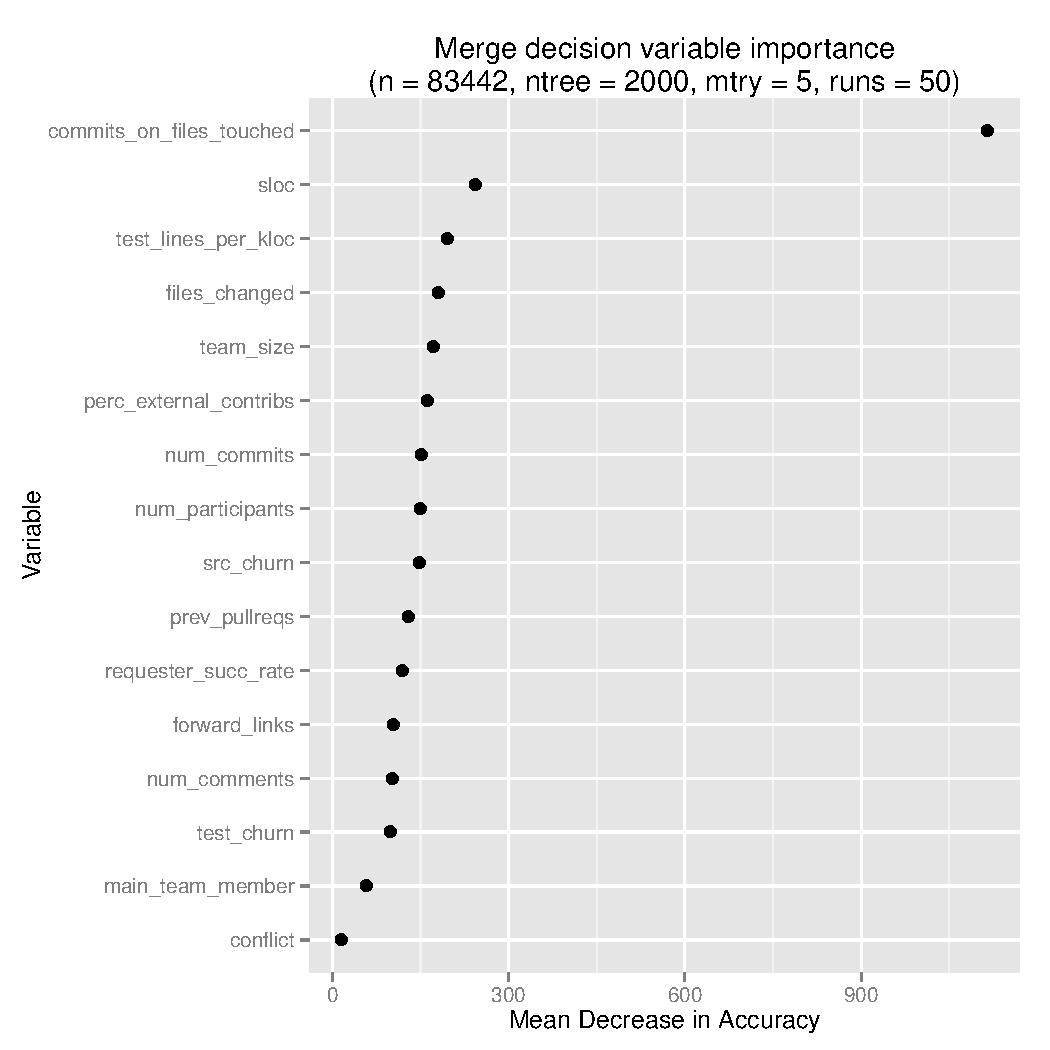
\includegraphics[scale=0.4]{varimp-merge-decision-83442-50.pdf} 
  \label{fig:varimp-merge-decision}
}
\subfigure{
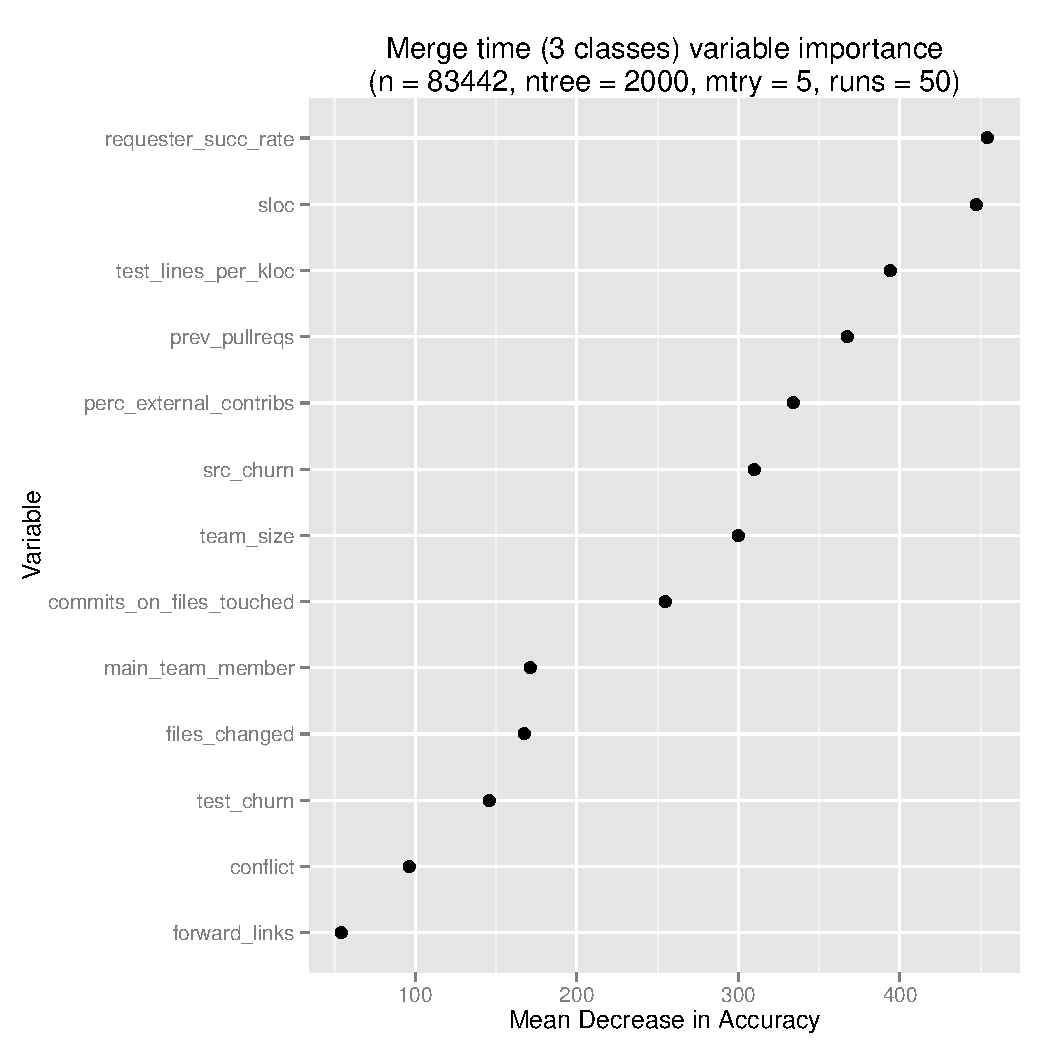
\includegraphics[scale=0.4]{varimp-merge-time-(3-classes)-83442-50.pdf}
  \label{fig:varimp-merge-time}
}
\caption{Random forest feature importance for predicting merge decision (a) and merge time (b)}
\label{fig:varimp}
\end{figure*}

To extract the features that are important for each classification task, we used
the process suggested by Genuer et al.~\cite{Genue10}. Specifically, we run the
algorithm 50 times on a randomly selected sample of $n = 83,442$ items, using a
large number of generated trees (2000) and trying 5 random variables per split.
We then used the mean across 50 runs of the  Mean Decrease in Accuracy metric,
as reported by the {\sc r} implementation of the random forest algorithm, to
evaluate the importance of each feature. The results can be seen in
Figure~\ref{fig:varimp}.

Finally, to validate our feature selection, we rerun the 10-fold
cross-validation process with increasing number of predictor features starting
from the most important one per case. In each iteration step, we add to the
model the next most important feature. We stop the process when the mean {\sc
auc} metric is within 2\% from the value in Table~\ref{tab:classif-perf} for
each task. The selected set of features should then be enough to predict the
classification outcome with reasonable accuracy, and therefore can be described
as important~\cite{Genue10}.

For the \textsf{mergedecision} task, the feature importance result is dominated
by the \texttt{commits\_\-on\_\-files\_\-touched} feature. By re-running the cross
validation process, we conclude that it suffices to use the features
 \texttt{commits\_\-on\_\-files\_\-touched}, \texttt{sloc} and \texttt{files\_changed}
to predict whether a pull request will be merged ({\sc auc:} 0.94, {\sc acc}:
0.86). Therefore, we can conclude that the decision to merge a pull request is
affected by whether it touches an actively developed part of the system (a
variation of the ``yesterday's weather'' hypothesis), how large the project's
source code base is and how many files the pull request changes.

%\fbox{
%\begin{minipage}{0.46\textwidth}
%\emph{RQ2: The three main factors that affect the decision to merge a pull request are: i)
%How active the area affect by the pull request has been recently ii) The size of the project iii) The number of files changed by the pull request.}
%\end{minipage}}

For the \textsf{mergetime} task, there is no dominant feature; the
classification model re-run revealed that at least 6 features are required to
predict how fast a pull request will be merged. The classification accuracy was
moderate ({\sc auc:} 0.74, {\sc acc}: 0.59), but still improved over random
selection. The results provide evidence that the developer's previous
track record, the size of the project and its test coverage and the project's
openness to external contributions seem to play a significant role on
how fast a pull request will be accepted.

%\fbox{
%\begin{minipage}{0.46\textwidth}
%\emph{RQ3: The three main factors that affect the time to merge a pull request
%are: i) The number of discussion comments ii) The size of the project iii) The
%project's test coverage.}
%\end{minipage}}

\noindent \fbox{ \begin{minipage}{0.46\textwidth} \emph{RQ3: The decision to
  merge a pull request is mainly influenced by whether the pull request modifies
  recently modified code. The time to merge is influenced by the developer's
  previous track record, the size of the project and its test coverage and the
  project's openness to external contributions.} \end{minipage}}

\section{Unmerged pull requests}

As most pull requests are indeed merged, it is interesting to explore why some
pull requests are \emph{not} merged. For that reason, we manually looked into 350 pull
requests and classified the reasons in categories as described in
Section~\ref{sec:qualdata}. The cross-validation of the categories on a
different set of pull requests revealed that the identified categories are
enough to classify all reasons for closing a pull request, even though
differences existed among the coders.  The results are presented in
Table~\ref{tab:unmerged}. 

The results show that there is no clearly outstanding reason for closing pull
requests. However, if we group together close reasons that have a timing
dimension (\textsf{obsolete}, \textsf{conflict}, \textsf{superseded}), we see
that 27\% of unmerged pull requests are closed due to concurrent modifications
of the code in project branches. Another 16\% (\textsf{superfluous},
\textsf{duplicate}, \textsf{deferred}) is closed as a result of the contributor
not having identified the direction of the project correctly and is therefore
submitting uninteresting changes. 10\% of the contributions are rejected with
reasons that have to do with project process and quality requirements
(\textsf{process}, \textsf{tests}); this may
be an indicator of processes not being communicated well enough or a rigorous
code reviewing process. Finally, another 13\% of the contributions are
rejected because the code review revealed an error in the implementation.

Moreover, for 15\% of the pull requests, the human examiners could not identify
the cause of not merging them. This usually means that there was no discussion
prior to closing the pull request or the pull request was automatically
initiated and managed by external tools; incidentally, all but one project that
had such pull requests in our random sample did not use Github's issue tracking
facilities. Consequently, the use of pull requests by such projects may be
superficial, only complementing parts of a process managed by other tools.
Finally, the human examiner could identify 19\% of the pull requests as merged
even though the automated heuristics could not; this means that the proportion
of merged pull requests reported in this study (84\%) may be slightly
underrated, due to non-inclusive heuristics. By extrapolation, the total number
of merged pull requests could be as high as 90\%.

It is interesting to note that only 13\% of the contributions are rejected due
to technical issues, which is the primary reason for code reviewing, while a
total 53\% are rejected for reasons having to do with the distributed nature of
the pull request process (concurrent modifications) or the way projects handle
communication of project goals and practices. This may mean that the pull-based
model (or at least the way Github implements it) may be transparent for the
project's core team~\cite{Dabbi13} but not so much for potential contributors. The fact that
human examiners could not understand why pull requests are rejected even after
manually reviewing them supports this hypothesis further.

\noindent
\fbox{
\begin{minipage}{0.46\textwidth}
  \emph{RQ4:  53\% of pull requests are rejected for reasons having to do with the
  distributed nature of pull based development.
  Only 13\% of the pull requests are rejected due to technical reasons.}
\end{minipage}}

\begin{table}[t]
  \begin{small}
  \centering
  \begin{tabular}{p{6em}p{18em}r}
    \hline
    \textbf{Reason} & \textbf{Description} & \textbf{\%}
\\
    \hline
    \textsf{obsolete} &	The {\sc pr} is no longer relevant, as the project
    has progressed. & 4\\

    \textsf{conflict} &	There feature is currently being implemented by other
    {\sc pr} or in another branch. & 5\\

    \textsf{superseded} &	A new {\sc pr} solves the problem better. & 18\\

    \textsf{duplicate} & The functionality already exists in the project. & 2 \\

    \textsf{superfluous} & {\sc pr} doesn't solve an existing problem or add a
    feature needed by the project. & 6 \\

    \textsf{deferred} & Proposed change delayed for further investigation in the
    future. & 8\\

    \textsf{process} & The {\sc pr} does not follow the correct project
    conventions for sending and handling pull requests. & 9\\
    
    \textsf{tests} & Tests failed to run. & 1\\

    \textsf{incorrect implementation} &	The implementation of the feature is
    incorrect, missing or not following project standards. & 13\\

    \hline 
    \textsf{merged} & The {\sc pr} was identified as merged by the human
    examiner & 19\\

    \textsf{unknown} & The {\sc pr} could not be classified due to lacking
    information & 15 \\

    \hline
  \end{tabular}
\end{small}
\caption{Reasons for closing pull requests without merging.}
\label{tab:unmerged}
\end{table}


\section{Discussion}
\label{sec:discussion}

\subsection{The pull-based development model}

\textbf{Development turnover.} One of the promises of the pull request model is
fast development turnover, i.e., the time between the submission of a pull
request and its acceptance in the project's main repository. In various studies
of the patch submission process in projects such as Apache and Mozilla, the
researchers found that the time to commit 50\% of the contributions to the main
project repository ranges from a few hours~\cite{Rigby08} to less than 3
days~\cite{Weiss08, Baysa12}. Our findings show that the majority (80\%) of pull
requests are merged within 4 days, 60\% in less than a day, while 30\% are
merged within one hour (independent of project size). These numbers are
indicating that pull-based development through pull requests may be more
efficient than traditional email-based patches.  Also, it is project-related
factors that affect the turnover time, rather than characteristics of the pull
request itself. This means that it is mostly up to the project to tune its processes
(notably, testing coverage and process openess) for faster turnover.

\textbf{Managing pull requests.} The interviewees in Dabbish et
al.~\cite{Dabbi13} identify the management of pull requests as the most
important project activity. Dabbish et al. mention that project managers ``made
inferences about the quality of a code contribution based on its style,
efficiency, thoroughness (for example, was testing included?), and the
submitter's track record''. Some of the inspection points mentioned by project
managers (testing code in
pull requests, track record) are also included as features in our classification
models, but they do not seem to affect the merge decision process as much.
However, the developer track record is important for the speed of processing
pull requests. Moreover, we found that from rejected pull requests, almost 53\%
are rejected due to the distributed nature of pull-based development. While the pull request process is
transparent from the project manager's side (and praised for that by Dabbish et
al.'s interviewees), our findings suggest it is less so from the potential contributor's point of view.

%\fbox{
%\begin{minipage}{0.46\textwidth}
%\emph{Pull requests are faster to merge than email-based patches. Projects can
%tune their reviewing and testing processes for faster turnover.}
%\end{minipage}}
%
\textbf{Attracting contributions.} Pham et al.~\cite{Pham13} mention
that pull requests make casual contributions straightforward through
a mechanism often referred to as ``drive-by commits''. As the
relative cost to fork a repository is negligible on Github (54\% of the
repositories are forks), it is not uncommon for developers to fork other
repositories to perform casual commits.
%, such as fixes to spelling mistakes or
%indentation issues. 
%In addition, Github provides web based editors
%for various file formats, by which any user can edit a file in another
%repository; behind the scenes, Github forks the repository and asks the user
%to create a pull request to the original one. 
Such commits might be identified
as pull requests that contain a single commit from users that are not yet part
of the project's community and comprise 7\% of the total number of pull
requests in 2012. Moreover, 3.5\% of the
forks were created for the sole purpose of creating a drive-by commit. More
work needs to be done for the accurate definition and assessment of the
implications of drive-by commits.

\textbf{Crowd sourcing the code review.}
An important part of the contribution process to an open source project is the
review of the provided code. Rigby and German~\cite{Rigby06},
report that 80\% of the core team members are also participating in the code
reviews for patches, a number that is also in line with earlier findings by
Mockus et al.~\cite{MOCKU02}. In our dataset, we found that \emph{all} core
team members across all projects have participated in at least
one discussion in a pull request. Moreover, we found that in \emph{all} projects
in our dataset, the community discussing pull requests is actually bigger
than the core team members.

%\fbox{
%\begin{minipage}{0.46\textwidth}
%\emph{Pull requests can help involve project community to the code review
%process.}
%\end{minipage}}
%
\textbf{Democratizing development.} One of the key findings of this work is
that pull requests are not treated differently based on their origin; both core
team members and external developers have equal chances to get their pull
request accepted within the same time boundaries. Indeed, even the
classification models we built assign to the corresponding feature low
importance. In our opinion, this is a radical change in the way open source
development is being carried out. Before pull requests, most projects employed
membership promotion strategies~\cite{Jense07} to promote interested third party
developers to the core team. With pull requests, developers can contribute to
any repository, without loss of authorship information. The chances that those
contributions will get accepted are higher with pull requests; across Github, more than 70\% of external contributions are merged
(40\% in other studies~\cite{Rigby06, Weiss08}). Specialized sites such as
Ohloh and CoderWall track developer activity and help developers advertise their
expertise. We believe that the democratization of the development effort will
lead to a substantially stronger commons ecosystem; this remains to be
verified in further studies.

\subsection{Implications}

\textbf{Contributors.} Prospective project contributors want their contributions
to be accepted. Our research shows that pull requests that affect parts of the
project that  have been changed often lately (are ``hot'') are very likely to
get merged. Also 80\% of the merged pull requests modify three or less files and
include patches less than 100 lines long. Therefore, our advice to contributors
seeking to add a particular feature or fix a bug is to ``keep it short''. If the
contribution's purpose is to make the contributor known to the project
community, it is also beneficial to affect a project area that is hot.

\textbf{Core team.} The primary job of the core team is to evaluate a list of
pull requests and decide whether to apply them or not. To make sure pull
requests are processed on time, the obvious strategy is to invest in a
comprehensive test suite and ensure that the project processes are sufficiently open and transparent. To avoid development concurrency related issues, core
team members could ask contributors to communicate their indented changes by
opening an issue that is then augmented by code and converted to a pull
request. The project should include a clear articulation of what is expected
from a pull request, for example tests or localized changes, on a prominent
location in the project's Github page.

% cd /cache && find . -type f -maxdepth 3|grep README.md|while read f; do if [ ! -z "`grep -i "pull request" $f`" ]; then echo $f; fi; done

%\textbf{Researchers.}
A direct application of our results is the construction of \emph{tools}
to help the core team prioritize their work; since we can predict
with very high accuracy whether a pull request will be merged or not, a
potential tool might suggest which pull requests can be merged without further
examination by the time they arrive. Other tools might examine the quality of
the pull request at the contributor's site, and based on the project's
profile, would provide automated suggestions for improvement (e.g., more tests,
documentation). 

\subsection{Threats to validity}

\textbf{Internal validity.} Our statistical analysis uses random forests as a way
to identify and rank cross-factor importance on two response variables. The classification
scores in the \textsf{mergetime} case are not perfect, so feature ranking may
not be exactly the same given a different dataset. Further work is needed on
validating the models on data from different sources (e.g., Bitbucket) or projects in different languages. 

To analyze the projects, we extracted data from i) the {\sc ght}orrent relational
database ii) the {\sc ght}orrent raw database iii) each project's Git repository.
Differences in the data abstraction afforded by each data source may
lead to different results in the following cases: 
i) Number of commits in a pull request: During their lifecycle, pull requests
may be updated with new commits. However, when developers use commit squashing,
the number of commits is reduced to one. Therefore the number of commits metric
used in our analysis is often an idealized version of the actual work
that took place in the context of a pull request.
ii) Number of files and commits on touched files: The commits reported
in a pull request also contain commits that merge branches, which the
developer may have merged prior to performing his changes. These commits
may contain several files not related to the pull request itself, which
in turn affects our results. Therefore, we  
filtered out those commits, but this may not reflect the contents of 
certain pull requests.

\textbf{External validity.} In our study, we used merged data from several
projects. The statistical analysis treated all projects as equal, even though
differences do exist.  For example, the larger project in our dataset, Ruby on
Rails, has more than 7,000 pull requests while the smaller ones 200.  While
we believe that the uniform treatment of the samples led to more robust results
in the classification experiment, variations in pull request handling among
projects with smaller core teams may be ironed out.  The fact that we performed
random selection cross-validation (instead of the more common sliding window
version) and obtained stable prediction results is, nevertheless,
encouraging.

\section{Related Work}

%Software development can be distributed across various
%di\-men\-sions~\cite{Gumm06}; among them, physical distribution distributes
%programming tasks across people collaborating remotely, while temporal
%distribution distributes tasks to people working in different time zones.
%Distribution of development activities has been initially thought to hinder
%collaboration~\cite{Herbs99, Batti01}, even though subsequent studies have
%shown that it does not pose significant threats to project
%quality~\cite{Spine06, Nguye08, Bird09a}. Access to online collaboration tools
%such as version control systems and bug databases have been identified as a necessary
%requirement for collaborative software development~\cite{Catal06}. Moreover, distributed collaboration on software artifacts can be
%facilitated through awareness building tools~\cite{Dabbi12, Lanza10}. 

Arguably, the first study of {\sc dvcs} systems as input for research was done
by Bird et. al in~\cite{Bird09}. One finding related to our work is that
maintaining authorship information leads to better identification of the
developer's contributions. Bird and Zimmermann~\cite{Bird12} investigated the
use of branches in {\sc dvcs}s (in Section~\ref{sec:bg}, we refer to this {\sc
dvcs} use as ``shared repository'') and found that excessive use of branching
may have a measurable, but minimal, effect on the project's time planning.
On the other hand, Barr et al.~\cite{Barr12} find that branches offer developers
increased isolation, even if they are working on inter-related tasks.
Finally, Shihab et al.~\cite{Shiha12} investigate the effect of branching on
software quality; they find that misalignment of branching structure and organizational structure is associated with higher post-release failure rates.

This work builds upon a long line of work on patch submission and acceptance.
In reference~\cite{MOCKU02}, Mockus et al. presented one of the first studies of
how developers interact on large open source projects in terms of bug reporting.
Bird et al.~\cite{Bird07a} introduced tools to detect patch submission and
acceptance in open source projects. Wei\ss gerber et al. presented an analysis
of patch submission, where they find that small patches are processed faster and
have higher change to be accepted into the repository. Baysal et
al.~\cite{Baysa12} find that 47\% of the total patches make it into the source
code repository, a number much lower than our finding for pull requests (84\%).
Jiang et al.~\cite{Jiang13} analyzed patch submission and acceptance on the
Linux kernel, which follows the pull-based development model in a more
decentralized and hierarchical manner. They find that the reviewing time is
becoming shorter through time while contributors can reduce it by controlling,
among others, the number of affected subsystems and by being more active in
their community. Those findings are similar to ours, where we find that the
contributor's previous track record and number of lines in the pull request
affect the time to merge it.

An inherent part of pull-based development is peer-reviewing the proposed
changes. In that sense, our work complements the work by Rigby and
Bird~\cite{Rigby13} and supports many of their findings. Both works find that
the peer review discussion is usually short, that peer-reviewed changes are
small and that reviews happen before the changes are committed and are very
frequent. Rigby and Bird's work examines industry-led projects and different
code reviewing processes than ours. The fact that many aspects of the results
are indeed similar leads us to hypothesize that it is the underlying
process (pull-based development) that govern the reviewing process.

Recently, Github has been the target of numerous publications. Dabbish
et.al~\cite{Dabbi13} found that Github's transparency helps developers manage
their projects, handle dependencies more effectively, reduce communication
needs, and decide what requires their attention. Peterson~\cite{Peter13}
finds that open source software ({\sc oss}) development on Github works mostly
similarly to traditional {\sc oss} development, with the exception of faster
turnaround times. Pham et al.~\cite{Pham13} examined the testing practices of
projects on Github and found that the lower barriers to submission hinders
high-quality testing as the work load on project member increases.  
Finally, McDonald and Goggins~\cite{McDon13} find that increased transparency in pull
requests allows allows teams to become more democratic in their decisions. 

\section{Conclusion}

The goal of this work is to obtain a deep understanding of the pull-based software development model, as used for many important open source projects hosted on Github. To that end, we have conducted a statistical analysis of millions of pull requests, as well of a carefully composed set of hunders of thousands of pull requests from projects actively using the pull-based model.

Our main findings are as follows:

\begin{enumerate}

  \item The pull-based model is not as popular as we had anticipated: Only 14\%
    of the active projects use pull requests, but this number is equal to the
    number of projects using the shared repository approach (Section 5).

  \item Most pull requests affect just a few dozen lines of code, and 60\% are
    processed (merged or discarded) in less than a day. The merge decision is
    \emph{not} affected by the presence of test code. Core members and external
    developers have equal chances to get their pull request accepted (Section
    6).

  \item The decision to merge is mainly affected by whether the pull request
    modifies recently modified code. The time to merge is influenced by various
    factors, including the developer's track record, and the project's test
    coverage.

  \item 53\% of non-merged pull requests are rejected for reasons related to the
    distributed nature of pull-based development. Only 13\% of the pull requests
    are rejected due to technical reasons.

\end{enumerate}

Our findings have the following implications:

\begin{enumerate}

  \item The pull-based model calls for a revision of some of our current
    understanding of open source software development. Iteresting research
    directions might include the formation of teams and management hierarchies,
    novel code reviewing practices and the motives of developers to work in a
    highly transparent workspace.

  \item Teams seeking to attract external contributors and to speed up merging
    of contributions can do so not just by providing clear pull request
    processing guidelines, but also by incorporating a high coverage test suite.

  \item Insufficient task articulation seems the most important cause for wasted
    (non-merged) work: Devising new ways for integrating task coordination into
    the pull-based model is a promising area of further research.

\end{enumerate}

Last but not least, our dataset provides a rich body of information on open source software development. The dataset as well as custom-built Ruby and R analysis tools are available on the Github repository 
\href{https://github.com/gousiosg/pullreqs}{gousiosg/pullreqs}, along with instructions on how to use them.

%We have presented an empirical investigation of how the pull-based development
%model works in practice. We explored its use on Github
%and then focused on the factors that affect pull request acceptance
%and processing time. This work makes the following contributions:
%
%\begin{itemize}
%
%  \item A statistical analysis of pull request usage on Github.
%   % We find increasing usage of pull requests through time.
%
%  \item A statistical analysis of several characteristics of pull requests.
%    %We
%    %find that pull requests are treated equally irrespective of whether they
%    %originate from the project's main team or the community, that projects are
%    %not getting faster at processing pull requests and that the inclusion of
%    %tests in a pull request does not directly affect whether it will be merged
%    %or not.
%
%  \item The main factors that affect pull request acceptance 
%    %(whether a pull
%    %request touches code that has been modified again recently) 
%    and processing
%    time.% (the developer's track record, the project's size and test coverage).
%  
%
%  \item The main factors for which pull requests are rejected
%    %, namely concurrent
%    %modifications among project branches and forks and incomplete understanding
%    %of the project's goals.
%
%  \item A carefully constructed dataset and a statistical toolkit for
%    performing analysis of the pull based development model.
%
%\end{itemize}
%
%This work is the first to explore the emerging paradigm of pull-based
%distributed software development. As such, while comprehensive, it is not complete.
%Further research can include the role and consequences of drive-by
%commits, the formation of teams and management hierarchies in a seemingly flat
%workspace, the role of testing in assessing pull request impact, large scale
%analysis of the reasons for pull request rejection, code reviewing practices,
%replications in more rigid work environments (e.g., companies) and tools for
%helping teams to automate the handling of pull requests.
%
%{\bfseries Replication} This study has been conducted using the {\sc ght}orrent
%dataset and custom-built Ruby and R tools. We share the tools, original data
%sources and extracted data files on the Github repository
%\texttt{gousiosg\-/\-pullreqs}, along with instructions on how to use them.
%
%\subsection*{Acknowledgements}

%We would like to thank the anonymous reviewers for their comments.
%This work is partially supported by Marie Curie {\sc ief} 298930 --- {\sc sefunc}.

\bibliographystyle{abbrv}
\balance
%\begin{small}

  \bibliography{pullreqs}
%\end{small}

\end{document}
